%%%%%%%%%%%%%%%%%%%%%%%%%%%%%%%%%%%%%%%%%%%%%%%%%%%%%%%%%%%%%%%%%%%%%%%%%%%%
%% Author template for Manufacturing & Service Operations Management (msom)
%% Mirko Janc, Ph.D., INFORMS, mirko.janc@informs.org
%% ver. 0.95, December 2010
%%%%%%%%%%%%%%%%%%%%%%%%%%%%%%%%%%%%%%%%%%%%%%%%%%%%%%%%%%%%%%%%%%%%%%%%%%%%
\documentclass[msom,nonblindrev]{informs3_arxiv} % current default for manuscript submission
%\documentclass[msom,nonblindrev]{informs3}

\usepackage{booktabs} % For formal tables
\usepackage[ruled,algo2e]{algorithm2e} % For algorithms
\renewcommand{\algorithmcfname}{ALGORITHM}
\SetAlFnt{\small}
\SetAlCapFnt{\small}
\SetAlCapNameFnt{\small}
\SetAlCapHSkip{0pt}
\IncMargin{-\parindent}

\usepackage{xurl}
\usepackage{graphicx}
% \usepackage{amsmath}
% \usepackage{amsfonts}
%\usepackage{amssymb}
% \usepackage{mathabx}
%\usepackage{amsthm}
% \usepackage{appendix}
\usepackage{algorithmicx}
\usepackage{algorithm}
\usepackage{algpseudocode} 
\usepackage{subfigure}
\usepackage[showdeletions]{color-edits}
\usepackage{caption}
\usepackage{paralist}
\usepackage{tikz-network}
\usepackage{hyperref}
\usepackage[noabbrev, capitalise]{cleveref}
%\usepackage{latex-macros-MSOM}
\usepackage{enumitem}
\usepackage{paralist}
\usepackage{booktabs}


%%\OneAndAHalfSpacedXI
\OneAndAHalfSpacedXII % Current default line spacing
%%\DoubleSpacedXII
% \DoubleSpacedXI

% If hyperref is used, dvi-to-ps driver of choice must be declared as
%   an additional option to the \documentclass. For example
%\documentclass[dvips,msom]{informs3}      % if dvips is used
%\documentclass[dvipsone,msom]{informs3}   % if dvipsone is used, etc.

% Private macros here (check that there is no clash with the style)

% % Natbib setup for author-year style
% \usepackage{natbib}
\usepackage[natbib, uniquename=false, uniquelist=false, maxcitenames=2,maxbibnames=4,style=authoryear]{biblatex}
 % \bibpunct[, ]{(}{)}{,}{a}{}{,}%
 \def\bibfont{\small}%
 \def\bibsep{\smallskipamount}%
 \def\bibhang{24pt}%
 \def\newblock{\ }%
 \def\BIBand{and}%
 \renewbibmacro*{in:}{% remove "In:"
  \iffieldundef{journaltitle}
    {}
    {\printtext{\bibstring{in}\intitlepunct}}}
  \renewbibmacro*{in:}{%  remove "In:"
  % \iffieldundef{journaltitle}
  %   {}  {\printtext{\bibstring{in}\intitlepunct}}
  }
 % \DeclareFieldFormat{title}{#1}
 \DeclareFieldFormat*{title}{#1} %remove "" from titles
 \renewbibmacro*{volume+number+eid}{%
  \printfield{volume}%
%  \setunit*{\adddot}% DELETED % remove dot between volume and issue number
  \setunit*{}% NEW (optional); there's also \addnbthinspace
  \printfield{number}%
  \setunit{\addcomma\space}%
  \printfield{eid}}
 \DeclareFieldFormat[article]{number}{\mkbibparens{#1}}
 \DeclareFieldFormat{pages}{#1} % remove pp.
 \renewcommand*{\bibpagespunct}{\addcolon\space} % add colon before page numbers.
\addbibresource{references.bib}


%% Setup of theorem styles. Outcomment only one. 
%% Preferred default is the first option.
\TheoremsNumberedThrough     % Preferred (Theorem 1, Lemma 1, Theorem 2)
%\TheoremsNumberedByChapter  % (Theorem 1.1, Lema 1.1, Theorem 1.2)

%% Setup of the equation numbering system. Outcomment only one.
%% Preferred default is the first option.
\EquationsNumberedThrough    % Default: (1), (2), ...
%\EquationsNumberedBySection % (1.1), (1.2), ...

% In the reviewing and copyediting stage enter the manuscript number.
%\MANUSCRIPTNO{} % When the article is logged in and DOI assigned to it,
                 %   this manuscript number is no longer necessary


\addauthor{mp}{red}
\addauthor{ar}{blue}
\newcommand\mar[1]{\arcomment{#1}}

\newcommand{\one}{\mathbf 1}
\newcommand{\zero}{\mathbf 0}
\newcommand{\FIX}{\mathsf{FIX}}
\newcommand{\SW}{\mathsf{SW}}
\newcommand{\linktoproof}[1]{\begin{center} \hyperref[#1]{\texttt{[Link to Proof]}}\end{center}}
\newcommand{\linktostatement}[1]{\begin{center} \hyperref[#1]{\texttt{[Link to Statement]}}\end{center}}
\newcommand{\ev}[2]{\mathbb E_{#1}\left [ #2 \right ]}
\newcommand{\crit}[0]{\mathsf{crit}}
\newcommand{\shrink}[0]{\vspace{-1em}}
\renewcommand{\Pr}{\mathbb P}

% \newtheorem{example}{Example}
% \newtheorem{assumption}{Assumption}
% \newtheorem{question}{Question}
% \newtheorem*{observation*}{Observation}
% \newtheorem*{definition*}{Definition}

% \theoremstyle{acmplain}
\newtheorem{informaltheorem}{Informal Theorem}

% Choose a citation style by commenting/uncommenting the appropriate line:
% \setcitestyle{acmnumeric}
% \setcitestyle{authoryear}

% \newenvironment{proofsketch}[1]{\begin{proof}[Proof Sketch]#1\end{proof}}
\newenvironment{proofsketch}{\paragraph{Proof Sketch.}}{\hfill$\qed$\medskip}

%%latex-macros
% mathcal letters
\newcommand{\cA}{\mathcal{A}}
\newcommand{\cB}{\mathcal{B}}
\newcommand{\cC}{\mathcal{C}}
\newcommand{\cD}{\mathcal{D}}
\newcommand{\cE}{\mathcal{E}}
\newcommand{\cF}{\mathcal{F}}
\newcommand{\cG}{\mathcal{G}}
\newcommand{\cH}{\mathcal{H}}
\newcommand{\cI}{\mathcal{I}}
\newcommand{\cJ}{\mathcal{J}}
\newcommand{\cK}{\mathcal{K}}
\newcommand{\cL}{\mathcal{L}}
\newcommand{\cM}{\mathcal{M}}
\newcommand{\cN}{\mathcal{N}}
\newcommand{\cO}{\mathcal{O}}
\newcommand{\cP}{\mathcal{P}}
\newcommand{\cQ}{\mathcal{Q}}
\newcommand{\cR}{\mathcal{R}}
\newcommand{\cS}{\mathcal{S}}
\newcommand{\cT}{\mathcal{T}}
\newcommand{\cU}{\mathcal{U}}
\newcommand{\cV}{\mathcal{V}}
\newcommand{\cW}{\mathcal{W}}
\newcommand{\cX}{\mathcal{X}}
\newcommand{\cY}{\mathcal{Y}}
\newcommand{\cZ}{\mathcal{Z}}

% mathbb letters
\newcommand{\Abb}{\mathbb{A}}
%\newcommand{\Bbb}{\mathbb{B}}
\newcommand{\Cbb}{\mathbb{C}}
\newcommand{\Dbb}{\mathbb{D}}
\newcommand{\Ebb}{\mathbb{E}}
\newcommand{\Fbb}{\mathbb{F}}
\newcommand{\Gbb}{\mathbb{G}}
\newcommand{\Hbb}{\mathbb{H}}
\newcommand{\Ibb}{\mathbb{I}}
\newcommand{\Jbb}{\mathbb{J}}
\newcommand{\Kbb}{\mathbb{K}}
\newcommand{\Lbb}{\mathbb{L}}
\newcommand{\Mbb}{\mathbb{M}}
\newcommand{\Nbb}{\mathbb{N}}
\newcommand{\Obb}{\mathbb{O}}
\newcommand{\Pbb}{\mathbb{P}}
\newcommand{\Qbb}{\mathbb{Q}}
\newcommand{\Rbb}{\mathbb{R}}
\newcommand{\Sbb}{\mathbb{S}}
\newcommand{\Tbb}{\mathbb{T}}
\newcommand{\Ubb}{\mathbb{U}}
\newcommand{\Vbb}{\mathbb{V}}
\newcommand{\Wbb}{\mathbb{W}}
\newcommand{\Xbb}{\mathbb{X}}
\newcommand{\Ybb}{\mathbb{Y}}
\newcommand{\Zbb}{\mathbb{Z}}

%%%%%%%%%%%%%%%%
\begin{document}
%%%%%%%%%%%%%%%%

% Outcomment only when entries are known. Otherwise leave as is and 
%   default values will be used.
%\setcounter{page}{1}
%\VOLUME{00}%
%\NO{0}%
%\MONTH{Xxxxx}% (month or a similar seasonal id)
%\YEAR{0000}% e.g., 2005
%\FIRSTPAGE{000}%
%\LASTPAGE{000}%
%\SHORTYEAR{00}% shortened year (two-digit)
%\ISSUE{0000} %
%\LONGFIRSTPAGE{0001} %
%\DOI{10.1287/xxxx.0000.0000}%

% Author's names for the running heads
% Sample depending on the number of authors;
% \RUNAUTHOR{Jones}
% \RUNAUTHOR{Jones and Wilson}
% \RUNAUTHOR{Jones, Miller, and Wilson}
% \RUNAUTHOR{Jones et al.} % for four or more authors
% Enter authors following the given pattern:
\RUNAUTHOR{Papachristou and Rahimian}

% Title or shortened title suitable for running heads. Sample:
% \RUNTITLE{Bundling Information Goods of Decreasing Value}
% Enter the (shortened) title:
\RUNTITLE{Production Networks Resilience}


% Enter the full title:
\TITLE{Production Networks Resilience: Cascading Failures, Power Laws and Optimal Interventions}

% Block of authors and their affiliations starts here:
% NOTE: Authors with same affiliation, if the order of authors allows, 
%   should be entered in ONE field, separated by a comma. 
%   \EMAIL field can be repeated if more than one author
\ARTICLEAUTHORS{%
\AUTHOR{Marios Papachristou}
\AFF{Cornell University, \EMAIL{papachristoumarios@cs.cornell.edu}, \URL{}}
\AUTHOR{M. Amin Rahimian}
\AFF{University of Pittsburgh, \EMAIL{rahimian@pitt.edu}, \URL{}}
% Enter all authors
} % end of the block

\ABSTRACT{%
\noindent{\bf Problem definition:}  The pandemic crisis made apparent the need to take a holistic view of production networks to understand risk factors that arise due to their many interdependent units. We investigate the structural factors contributing to the severity of cascading failures in production networks, how to quantify the effect of these risk factors with resilience metrics, and how to design and evaluate interventions to improve resilience. 

%The pandemic crisis made apparent the need to take a holistic view of production networks for understanding risk factors that arise as a result of many interdependent units. In this paper, we investigate the structural factors that contribute to the severity of cascading failures in supply chain networks, how to quantify the effect of these risk factors, and how to design and evaluate interventions to mitigate these risk factors. %The pandemic crisis made apparent the need to take a holistic view of production networks for understanding risk factors that arise as a result of many interdependent units. In this paper, we investigate the structural factors that contribute to the severity of cascading failures in supply chain networks and 
    
   
\noindent{\bf Methodology/Results:} 
We propose a node percolation process on production networks that models product suppliers failing independently due to exogenous, systemic shocks and causing other products to fail as their production requirements are unmet. We first show that the size of the cascading failures follows a power law in random directed acyclic graphs, whose topology encodes the natural ordering of products from simple raw materials to complex products. This motivates the need for a resilience metric, which we define as the maximum magnitude shock the production network can withstand with only a small fraction of products failing. Next, we study the resilience of several architectures, such as trees, parallel products, and random trellis, and classify them as resilient or fragile depending on their topological attributes. In the next step, we give general lower bounds and optimal interventions for improving resilience as a function of Katz centralities. Finally, we empirically calculate the resilience metric and study interventions in various real-world networks to validate our theoretical results.
% defined by a node percolation process corresponding to product suppliers failing independently due to systemic shocks. 
% We first show that the size of the cascades follows a power law in random directed acyclic graphs, whose topology encodes the natural ordering of products from simple raw materials to complex products. This motivates the need for a supply chain resilience metric, which we define as the maximum magnitude shock that the production network can withstand such that at least $(1 - \varepsilon)$-fraction of the products are produced with high probability as the size of the production network grows to infinity. Next, we study the resilience of many network architectures and classify them as resilient, where large cascading failures can be avoided almost surely, and fragile, where large cascades are inevitable. In the next step, we give bounds on the expected size of cascading failures in a given production network graph as the solution to a linear program and show that extending the node percolation process to a joint percolation process that affects the nodes and the links of the production network becomes a special instance of the well-studied financial contagion model of Eisenberg and Noe. We show that under certain assumptions, the Katz centrality of each node can be used as a measure of their vulnerability and give general lower bounds as well as optimal interventions for improving resilience as a function of Katz centralities. Finally, to validate our theoretical results, we empirically calculate the resilience metric and study interventions in a variety of real-world networks.

% as the solution to a linear program and show that extending the node percolation process to a joint percolation process that affects the nodes and the links of the production network becomes a special instance of the well-studied financial contagion model of Eisenberg and Noe. We

% propose a linear program to bound the expected size of cascading failures in general graphs and show that under certain assumptions, the Katz centrality of each node can be used as a measure of their vulnerability and

\noindent {\bf Managerial implications:} We offer new thoughts and theories on reasoning about supply chain resilience based on topological attributes such as source dependency and product complexity and propose novel, theory-informed metrics that we evaluate empirically on real-world networks. Our theories also inform intervention designs for improving resilience, not just from a firm’s perspective but also on a national scale.

%networks and can explicitly measure how different factors such as number of required inputs and supplier affect production affect network resilience differently

%We propose a theory-informed resilience metric that reflects the effect of different topological factors, such as network width and depth, and give optimal intervention designs for increased resilience. We also give empirical evidence for the utility of our metrics to measure resilience not just from the perspective of a firm or an industry but also on national scales. We offer new thoughts and theories about how to reason about supply chain resilience based on topological attribute such as network width and depth, and propose theory-informed metrics that are quantifiable on real-world supply chain networks and can explicitly measure how factors such as number of required inputs and supplier affect production network resilience.  
}%

% Sample
%\KEYWORDS{deterministic inventory theory; infinite linear programming duality; 
%  existence of optimal policies; semi-Markov decision process; cyclic schedule}

% Fill in data. If unknown, outcomment the field
\KEYWORDS{Production networks, Resilience, Cascading failures, Interventions}
\HISTORY{First Version: March 22, 2023. This version: \today.}

\maketitle
%%%%%%%%%%%%%%%%%%%%%%%%%%%%%%%%%%%%%%%%%%%%%%%%%%%%%%%%%%%%%%%%%%%%%%

% Samples of sectioning (and labeling) in MSOM
% NOTE: (1) \section and \subsection do NOT end with a period
%       (2) \subsubsection and lower need end punctuation
%       (3) capitalization is as shown (title style).
%
%\section{Introduction.}\label{intro} %%1.
%\subsection{Duality and the Classical EOQ Problem.}\label{class-EOQ} %% 1.1.
%\subsection{Outline.}\label{outline1} %% 1.2.
%\subsubsection{Cyclic Schedules for the General Deterministic SMDP.}
%  \label{cyclic-schedules} %% 1.2.1
%\section{Problem Description.}\label{problemdescription} %% 2.

% Text of your paper here
\begin{refsection}
\section{Introduction}
\label{sec:introduction}
% \begin{itemize}
%     % Diffusion of FL
%     \item {\st{Diffusion of FL}}
%     % Security threats to FL
%     \item {\st{Security threats to FL with particular focus on model poisoning}}
%     % Limitations of existing countermeasures
%     \item {\st{Current countermeasures (e.g., KRUM) and their limitations}}
%     % Proposed method and its advantages
%     \item {\st{Intuitive description of the proposed method and its difference (i.e., advantages) w.r.t. state of the art}}
%     % Main contributions
%     \item {\st{Summary of the main contributions of this work}}
%     % Paper's structure and organization
%     \item {\st{Paper's structure and organization}}
% \end{itemize}

% Diffusion of FL
Recently, {\em federated learning} (FL) has emerged as the leading paradigm for training distributed, large-scale, and privacy-preserving machine learning (ML) systems~\cite{mcmahan2017googleai,mcmahan2017aistats}. 
The core idea of FL is to allow multiple edge clients to collaboratively train a shared, global model without disclosing their local private training data.
%Specifically, an FL system consists of a central server and many edge clients; 
A typical FL round involves the following steps: {\em(i)} the server randomly picks some clients and sends them the current, global model; {\em(ii)} each selected client locally trains its model with its own private data; then, it sends the resulting local model to the server;\footnote{Whenever we refer to global/local model, we mean global/local model {\em parameters}.} {\em(iii)} the server updates the global model by computing an \emph{aggregation function}, usually the average (FedAvg), on the local models received from clients.
% \begin{enumerate}
%     \item[{\em(i)}] the server sends the current, global model to the clients and appoints some of them for training;
%     \item[{\em(ii)}] each selected client locally trains its copy of the global model with its own private data; then, it sends the resulting local model back to the server;\footnote{Whenever we refer to global/local model, we mean global/local model {\em parameters}.}
%     \item[{\em(iii)}] the server updates the global model by computing an \emph{aggregation function} on the local models received from clients (by default, the average, also referred to as FedAvg~\cite{mcmahan2017aistats}).
% \end{enumerate}
This process goes on until the global model converges. %(e.g., after a certain number of rounds or other similar stopping criteria).
%\\
% The advantages of FL over the traditional, centralized learning paradigm are undoubtedly clear in terms of flexibility/scalability (clients can join/disconnect from the FL network dynamically), network communications (only model weights\footnote{We will use \textit{parameters} and \textit{weights} interchangeably.} are exchanged between clients and server), and privacy (each client's private training data is kept local at the client's end and not uploaded to the server).
\\
% Security threats to FL
%However, the growing adoption of FL also raises security concerns~\cite{costa2022covert}, particularly about its confidentiality, integrity, and availability.
Although its advantages over standard ML, FL also raises security concerns~\cite{costa2022covert}. %, particularly about its confidentiality, integrity, and availability~\cite{costa2022covert}.
% OLD, LONG VERSION
% Indeed, some work deals with privacy leakage that may expose the local data of some clients~\cite{melis2019sp}. 
% A large body of work, instead, investigates attacks that usually aim to detriment the predictive accuracy of the learned global model. For instance, \emph{data poisoning} attacks achieve this goal by letting an adversary pollute the training set of some corrupt FL clients with maliciously crafted examples~\cite{jagielski2018sp}.
% Similarly, in \emph{model poisoning} the attacker attempts to tweak the global model weights~\cite{bhagoji2019pmlr} by directly perturbing the local model's weights of some infected FL clients before these are sent to the central server for aggregation, usually via so-called Byzantine attacks. 
% It turns out that Byzantine model poisoning attacks severely impact standard FedAvg; therefore, more robust aggregation functions must be designed to make FL systems secure.
Here, we focus on \emph{untargeted model poisoning} attacks~\cite{bhagoji2019pmlr}, where an adversary attempts to tweak the global model weights %\footnote{We will use the terms \textit{parameters} and \textit{weights} interchangeably.} 
by directly perturbing the local model's parameters of some infected clients before these are sent to the central server for aggregation.
In doing so, the adversary aims to jeopardize the global model \textit{indiscriminately} at inference time.
Such model poisoning attacks severely impact standard FedAvg; therefore, more robust aggregation functions must be designed to secure FL systems.
\\
% In this paper, we focus on designing a novel robust aggregation scheme at the server's end to contrast the effect of Byzantine model poisoning attacks.
%
% Current countermeasures and their limitations
%Several countermeasures have been proposed in the literature to combat model poisoning attacks on FL systems.
% Some methods use simple statistics more robust than plain average to smooth the impact of malicious updates (e.g., Trimmed Mean and FedMedian~\cite{yin2018icml}). 
% Other defenses implement outlier detection techniques to discard malicious updates from the aggregation performed at the server's end. Those are either based on heuristics (e.g., Krum/Multi-Krum~\cite{blanchard2017nips} and Bulyan~\cite{mhamdi2018pmlr}) or data-driven approaches (e.g., K-means clustering~\cite{shen2016acm} or DnC via spectral analysis~\cite{shejwalkar2021ndss}). 
% Finally, some strategies rely on a centralized ``source of trust'' to spot potential malicious updates (e.g., FLTrust~\cite{cao2020fltrust}).
% Several countermeasures have been proposed in the literature to combat model poisoning attacks on FL systems, i.e., to discard possible malicious local updates from the aggregation performed at the server's end. 
% These techniques range from simple statistics more robust than plain average (e.g., Trimmed Mean and FedMedian~\cite{yin2018icml}) to outlier detection heuristics (e.g., Krum/Multi-Krum~\cite{blanchard2017nips} and Bulyan~\cite{mhamdi2018pmlr}) or data-driven approaches (e.g., spectral analysis via K-means clustering~\cite{shen2016acm} or spectral analysis), or methods based on ``source of trust'' (e.g., FLTrust~\cite{cao2020fltrust}).
% OLD, LONG VERSION
%Several countermeasures have been proposed in the literature to combat Byzantine model poisoning attacks on FL systems.
% Descriptive statistics
% For example, Trimmed Mean and FedMedian aggregate local model updates using more robust statistics than standard average~\cite{yin2018icml}.
%
% % Heuristics for outlier detection
% Many existing Byzantine-resilient strategies implement some outlier detection heuristics to discard the model updates sent by potentially malicious clients from the input of the aggregation function.
% One of the most popular heuristics is Krum~\cite{blanchard2017nips}.
% This strategy tries to mitigate the impact of Byzantine attacks by selecting as a global model the local model with the smallest sum of Euclidean distances to {\em all} the other local models.
% Although powerful, Krum requires the server to know (or, at least, estimate) the number of malicious FL clients upfront, which is generally impossible in a realistic attack scenario. %
% Moreover, Krum may become ineffective for complex, high-dimensional model parameter spaces due to the curse of dimensionality.
% Bulyan~\cite{mhamdi2018pmlr} tries to overcome this issue by combining Krum with a variant of Trimmed Mean.
% % Data-driven outlier detection
% Other strategies use data-driven outlier detection techniques -- e.g., via K-means clustering~\cite{shen2016acm} -- to spot potential malicious local model updates. 
% %For instance, Shen et al. propose to cluster local model updates with K-means and thus identify outliers.
%
% % Other techniques
% As far as the server is concerned, any local model received can be from a potential malicious client. 
% FLTrust~\cite{cao2020fltrust} assumes the server acts as a client, i.e., trains a local model on an additional {\em trustworthy} dataset at the server's end and compares it against all the local models from other clients. 
% This way, the server can rely on some ``source of trust'' when discarding potentially malicious clients.
%\\
% Limitations of existing Byzantine-resilient strategies
Unfortunately, existing defense mechanisms either rely on simple heuristics (e.g., Trimmed Mean and FedMedian by~\cite{yin2018icml}) or need strong and unrealistic assumptions to work effectively (e.g., foreknowledge or estimation of the number of malicious clients in the FL system, as for Krum/Multi-Krum~\cite{blanchard2017nips} and Bulyan~\cite{mhamdi2018pmlr}, which, however, cannot exceed a fixed threshold).
Furthermore, outlier detection methods using K-means clustering~\cite{shen2016acm} or spectral analysis like DnC~\cite{shejwalkar2021ndss} do not directly consider the temporal evolution of local model updates received.
Finally, strategies like FLTrust~\cite{cao2020fltrust} require the server to collect its own dataset and act as a proper client, thereby altering the standard FL protocol.
\\
% OLD, LONG VERSION
% Overall, existing Byzantine-resilient strategies are either simple heuristics (e.g., FedMedian) or, if they are more complex, they rely on strong and unrealistic assumptions to work effectively (e.g., knowing the number of malicious clients in the FL system in advance, as for Krum and alike).
% Furthermore, data-driven outlier detection methods do not consider the temporary evolution of local model updates received (e.g., K-means clustering). 
% Finally, strategies like FLTrust requires the server to collect its own dataset and act as a proper client, thereby altering the standard FL protocol.
%
% Description of the proposed method
This work introduces a novel pre-aggregation \textit{filter} robust to untargeted model poisoning attacks. Notably, this filter $(i)$ operates without requiring prior knowledge or constraints on the number of malicious clients and $(ii)$ inherently integrates temporal dependencies. 
The FL server can employ this filter as a preprocessing step before applying \textit{any} aggregation function, be it standard like FedAvg or robust like Krum or Bulyan.
Specifically, we formulate the problem of identifying corrupted updates as a multidimensional (i.e., matrix-valued) time series anomaly detection task. 
The key idea is that legitimate local updates, resulting from well-calibrated iterative procedures like stochastic gradient descent (SGD) with an appropriate learning rate, show \textit{higher predictability} compared to malicious updates. This hypothesis stems from the fact that the sequence of gradients (thus, model parameters) observed during legitimate training exhibit regular patterns, as validated in Section~\ref{subsec:intuition}. %until convergence. 
%This regularity may be more pronounced for smooth convex loss functions, but it can still be captured within an appropriate time window, even for more complex and convoluted loss surfaces. 
%We provide evidence of this claim in Appendix~B, where we show that the average mutual information (i.e., ``predictability''), calculated over pairs of legitimate model updates sent at different FL rounds, is significantly higher than the corresponding computation for a malicious client.
\\
Inspired by the matrix autoregressive (MAR) framework for multidimensional time series forecasting~\cite{chen2021je}, we propose the FLANDERS ({\em \textbf{F}ederated \textbf{L}earning meets \textbf{AN}omaly \textbf{DE}tection for a \textbf{R}obust and \textbf{S}ecure}) filter.
The main advantages of FLANDERS over existing strategies like FLDetector~\cite{zhao2020multivariate} are its resilience to large-scale attacks, where $50\%$ or more FL participants are hostile, and the capability of working under realistic non-iid scenarios.
We attribute such a capability to two key factors: $(i)$ FLANDERS works without knowing a priori the ratio of corrupted clients, and $(ii)$ it embodies temporal dependencies between intra- and inter-client updates, quickly recognizing local model drifts caused by evil players. Below, we summarize our main contributions:

\begin{itemize}
\item[{\em(i)}]
We provide empirical evidence that the sequence of models sent by legitimate clients is more predictable than those of malicious participants performing untargeted model poisoning attacks.
\\
\item[{\em(ii)}] 
We introduce FLANDERS, the first pre-aggregation filter for FL robust to untargeted model poisoning based on multidimensional time series anomaly detection.
\\
\item[{\em(iii)}] 
We integrate FLANDERS into Flower,\footnote{\scriptsize{\url{https://flower.dev/}}} a popular FL simulation framework for reproducibility.
\\
\item[{\em(iv)}] 
We show that FLANDERS improves the robustness of the existing aggregation methods under multiple settings: different datasets, client's data distribution (non-iid), models, and attack scenarios.
\\
\item[{\em(v)}] 
We publicly release all the implementation code of FLANDERS along with our experiments.\footnote{\scriptsize{\url{https://anonymous.4open.science/r/flanders_exp-7EEB}}}
\end{itemize}

% Paper's structure and organization
The remainder of the paper is structured as follows. %some related work and the current state-of-the-art solutions to security issues that FL entails. 
Section~\ref{sec:background} covers background and preliminaries. 
In Section~\ref{sec:related}, we discuss related work.
Section~\ref{sec:problem} and Section~\ref{sec:method} describe the problem formulation and the method proposed. % to tackle it. 
Section~\ref{sec:experiments} gathers experimental results. %, and Section~\ref{sec:limitations} discusses some limitations of this work.
Finally, we conclude in Section~\ref{sec:conclusion}.
 %discusses the limitations of this work and draws future research directions.
%reports conclusions and draws perspectives for future research directions.

%%%%%%% OLD %%%%%%%
%to overcome the resilience of Byzantine failures in distributed Stochastic Gradient Descent computations. 
% The strength of Krum is its time complexity, which is linear in the gradient dimension. 
% However, the robustness of the approach is guaranteed for gradient-based learning applications only when the majority of the clients are not compromised. 
% Besides, the aggregation mechanism of Krum, as well as that of similar methods, is robust from a coarse-grained perspective and does not provide solutions to errors and perturbations that may occur at inference time.
%A related approach to~\cite{blanchard2017nips} is the work of Su et al.~\cite{su2016dc}. Here, the authors propose an iterated approximate agreement to tackle a multi-layer scenario attacked by Byzantine agents. 
%However, the method works efficiently on the sole discrete context and it is inapplicable to continuous state environments.
%\gabri{Maybe, we should just talk about the main limitations of existing countermeasures without digging into their details (or, we can just mention Krum as this is the most popular one). I will move the description of all these methods to the Related Work section.}
\section{The Production Network} \label{sec:preliminaries}

\begin{figure}[t]
    \centering
    \subfigure[Production Network \label{subfig:product_graph}]{
    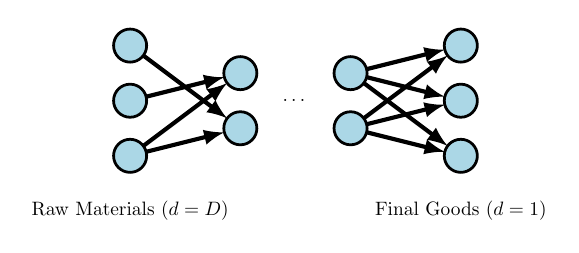
\begin{tikzpicture}[transform shape,scale=0.7]
        \Vertex[x=-1, y=-1]{u1}
        \Vertex[x=-1, y=0]{u2}
        \Vertex[x=-1, y=1]{u3}
        \Text[x=-1, y=-2, fontsize=\normalsize]{Raw Materials ($d = D$)}

        \Vertex[x=1, y=-0.5]{v1}
        \Vertex[x=1, y=0.5]{v2}
        

        \Edge[Direct, color=black](u1)(v1)
        \Edge[Direct, color=black](u3)(v1)
        
        \Edge[Direct, color=black](u2)(v2)
        \Edge[Direct, color=black](u1)(v2)
        
        \Text[x=2, y=0]{$\dots$}
        
        \Vertex[x=5, y=-1]{w1}
        \Vertex[x=5, y=0]{w2}
        \Vertex[x=5, y=1]{w3}
        \Text[x=5, y=-2, fontsize=\normalsize]{Final Goods ($d = 1$)}
        
        \Vertex[x=3, y=0.5]{z1}
        \Vertex[x=3, y=-0.5]{z2}
        
        \Edge[Direct, color=black](z1)(w1)
        \Edge[Direct, color=black](z1)(w2)
        \Edge[Direct, color=black](z1)(w3)
        
        \Edge[Direct, color=black](z2)(w1)
        \Edge[Direct, color=black](z2)(w2)
        \Edge[Direct, color=black](z2)(w3)
        
        
    \end{tikzpicture}}
    \subfigure[Supply Chain Network Between Two Products \label{subfig:supply_chain}]{
    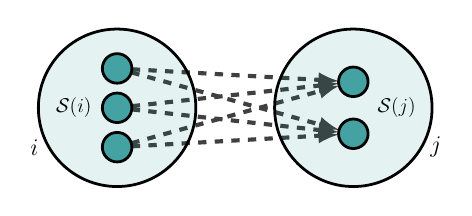
\begin{tikzpicture}[transform shape,scale=0.5]
    
    \Vertex[x=0, y=0, color=teal, opacity=0.1, size=4]{i}
    \Vertex[x=0, y=0, color=teal, opacity=0.7, size=0.75]{Si1}
    \Vertex[x=0, y=1, color=teal, opacity=0.7, size=0.75]{Si2}
    \Vertex[x=0, y=-1, color=teal, opacity=0.7, size=0.75]{Si3}

    \Text[x=-2.1,y=-1,fontsize=\LARGE]{$i$}
    \Text[x=8.1,y=-1,fontsize=\LARGE]{$j$}

    \Text[x=-1.1, y=0,fontsize=\Large]{$\cS(i)$}

    \Text[x=7.1, y=0,fontsize=\Large]{$\cS(j)$}


    \Vertex[x=6, y=0, color=teal, opacity=0.1, size=4]{j}
    \Vertex[x=6, y=-0.66, color=teal, opacity=0.7, size=0.75]{Sj1}
    \Vertex[x=6, y=0.66, color=teal, opacity=0.7, size=0.75]{Sj2}

    \Edge[Direct,style=dashed](Si1)(Sj1)
    \Edge[Direct,style=dashed](Si1)(Sj2)

    \Edge[Direct,style=dashed](Si2)(Sj1)
    \Edge[Direct,style=dashed](Si2)(Sj2)

    \Edge[Direct,style=dashed](Si3)(Sj1)
    \Edge[Direct,style=dashed](Si3)(Sj2)
    
    \end{tikzpicture}}
    \caption{Supply Chain Instance. Each node in the production network of \cref{subfig:product_graph} has a supplier set. The supply chain network between two products is shown in \cref{subfig:supply_chain}.}

    \label{fig:supply_chain}
\end{figure}


We start by describing the production network (see \cref{subfig:product_graph} for an example production network).  We consider the production of a set of products $\cK$ with cardinality $|\cK| = K$ where each product $i \in \cK$ can be produced by a number of suppliers and also requires certain inputs to be produced. Specifically, each product $i \in \cK$ has a set of requirements (inputs), denoted by $\cN(i)$ that it needs in order to be made. The products and the set of requirements for each product define \emph{production network} $\cG(\cK, \cE)$. The production network is also associated with the adjacency matrix $A$ and the cardinality of the edges is $M = |\cE|$.  

The production network $\cG$ starts with \emph{raw materials} (or sources), which are materials that do not require any input, that is, they have $|\cN(i)| = 0$ and are the ``initial products'' that are used in the production of others. We denote the set of raw materials (or primary sector), which corresponds to products that do not have input, by $\cR$ and its cardinality by $|\cR| = r$. We use $\cC$ to denote the set of final goods (or final sector), which corresponds to products that do not have output, and use $c = |\cC|$ to denote their cardinality. Each product $i \in \cK$ can be sourced from a set of suppliers $\cS(i)$. We assume that a supplier of a product can source from any of the suppliers of the products on which it depends.

% (one may argue here that it is impossible that every supplier of a product $i$ can source from every supplier of, say, product $j$, due to geographical constraints. The issue can be mitigated by expanding vertex $j$ to multiple sub-nodes).

We define the sourcing dependency $m$ of $\cG$ as the maximum in-degree of any product, and the supply dependency $\mu$ of $\cG$ as the maximum out-degree of any product. If $\cG$ is random, $m$ and $\mu$ are defined to be the corresponding expected in/out-degrees. 
 
Associated with the production network $\cG$, we can also define a supply chain network by focusing on the supply relations between the suppliers of different products (cf. \cref{subfig:supply_chain}). The supply chain network $\cH$ is defined as a graph with vertex set $\cV(\cH) = \bigcup_{i \in \cK} \cS(i)$ and edge set $\cE(\cH) = \bigcup_{i \in \cK} \bigcup_{j \in \cN(i)} \cB(\cS(i), \cS(j))$, where $\cB(\cS(i), \cS(j))$ is the complete bipartite graph between $\cS(i)$ and $\cS(j)$.  

% \xpar{Structural Assumptions on $\cG$.} For our main results, we make the structural assumption that the production network $\cG$ is a Directed Acyclic Graph (DAG), i.e., a natural order exists among the products being produced, i.e., the production of more complex products depends on sourcing inputs from simpler products. Such an assumption has appeared in prior work, e.g., \citet{elliott2022supply,blaettchen2021traceability,bimpikis2019supply}. Later in the paper (\cref{sec:general_supply_chains}), we show how we can relax this assumption and allow for cycles in $\cG$.

\xpar{Example} Assume a simple network that produces $\cK = \{  \text{engines}, \text{bolts}, \text{screws} \}$. We have, e.g., $\cN(\text{engines}) = \{ \text{bolts}, \text{screws} \}$ and $\cS(\text{engines}) = \{ \text{BMW}, \text{General Motors} \}$, and suppliers for the screws and bolts.

\xpar{Additional notation} We use $[K]$ to denote the set $\{ 1, \dots, K \}$. 
For vectors (resp. matrices), we use $\| v \|_p$ (resp. $\| V \|_p$) for the $p$-norm of $v$ (resp. for the induced $p$-norm); for the Euclidean norm (i.e., $p = 2$), we omit the subscript. $\zero$ (resp. $\one$) denotes the column vector of all zeros (resp. all ones) and $\one_S$ represents the column vector indicator of the set $S$. 
We use $x \wedge y$ (resp. $x \vee y$) as shorthand for the coordinate-wise minimum (resp. maximum) of the vectors $x$ and $y$.
Finally, order relations $\ge, \le, >, <$ denote coordinate-wise ordering. We use $\cG^R$ to denote the edge-reversed graph of $\cG$, i.e., the graph which has the same vertex set as $\cG$ and reversed edges. In our context, $\cG$ corresponds to the graph of supply relations and $\cG^R$ corresponds to the graph of source relations. The notation $x_n \asymp y_n$ means that $\lim_{n \to \infty} \frac {x_n} {y_n} = 1$. 


% \mpcomment{talk about modelling assumptions on the production network and how they can model a wide range of phenomena such as geographically separate groups of suppliers}

\subsection{Node Percolation in the Homogeneous Model} \label{sec:node_percolation}

For most of the theoretical results of this paper, we focus on the homogeneous failure model for simplicity of exposition. The \textbf{homogeneous} model assumes that all nodes have the \textit{same number of suppliers} and all products \textit{fail independently} of each other with the same probability.  Later in the paper (see \cref{sec:heterogeneities}), we introduce the \textbf{heterogeneous} model, which assumes that failures \textit{can be correlated with each other}, as well as each product, can have a different number of suppliers. 

According to the homogeneous model, each product $i$ has a \textit{constant} number of suppliers that is equal to $n$. The supply chain graph $\cG$ undergoes a node percolation process in which each supplier fails independently at random with probability $x \in (0, 1)$. Each product can be produced if, and only if, \emph{(i)} all of its requirements $j \in \cN(i)$ can be produced, and, \emph{(ii)} at least one of the suppliers $s \in \cS(i)$ is operational. Upon completion of the percolation process, a random number $F$ of products fails, and the remaining $S = K - F$ products survive. The number of surviving products can be expressed as $S = \sum_{i \in \cK} Z_i$ where $\{ Z_i \}_{i \in \cK}$ are the indicator variables that equal to one if, and only if, product $i$ is produced and are zero otherwise. The sequence of variables $\{ Z_i \}_{i \in \cK}$ obeys the following random system of equations (or dynamics) for every $i \in \cK$:
\begin{align} \label{eq:dynamics} 
    Z_i & = \prod_{j \in \cN(i)} Z_j \left ( 1 - \prod_{s \in \cS(i)} X_{is} \right ), 
\end{align} where $X_{is} \overset  {\mathsf{i.i.d.}} {\sim} \mathrm{Be}(x)$ correspond to the indicator variables that equal to 1 if supplier $s \in \cS(i)$ of product $i \in \cK$ has spontaneously failed.  Our paper aims to study the random behavior of $F$ (resp. $S$). A planner is interested in finding the maximum probability value $x$ such that the number of failures is at most $\varepsilon K$ (e.g., sublinear) with high probability. We show that some very simple production networks can experience power-law cascades to motivate such a resilience metric. 

\subsection{Motivation for a resilience metric: cascading failures and the emergence of power laws in random DAG structures} \label{sec:motivation}

We start by motivating the need for the definition of a resilience measure for supply chain graphs. More specifically, similar to large social networks \citep{leskovec2007patterns,wegrzycki2017cascade} and power networks \citep{dobson2004branching,dobson2005loading,nesti2020emergence}, we show that a randomly generated supply chain with random DAG structure exhibits cascade sizes that obey a power law, namely the average cascade size is dominated by a few very large cascades rather than the many smaller ones. Our motivation comes from the literature on network science and social networks literature in accordance with the literature that uses network science ideas to introduce and study supply chain concepts (see, e.g., \cite{borgatti2009social,artime2024robustness,perera2017network}).

In a supply chain, we can assume that there is a ``natural order'' among the products being produced; namely, producing more complex products is contingent on the supply of simpler products. In a supply chain, raw materials and component parts are typically transformed into intermediate products and finished products through a series of production processes. The production of more complex products often depends on the availability of simpler products, as the simpler products are used as inputs in the production of the more complex products. For example, in the production of a car, the production of the car's engine may depend on the availability of simpler components, such as computer chips. In its simplest form, this behavior can be captured by a random DAG model, where a DAG is created by independently sampling edges via coin tosses. We also want to emphasize that the random DAG model has a significantly different structure from the Erd\"os-R\'enyi random graph, which allows the study of cascading behavior.

%Similarly, the production of the car's body may depend on the availability of the car's engine, as well as other intermediate products such as doors and windows.  

To observe this, we start with the random DAG model $\mathsf{rdag}(K, p)$ described in the work of \citet{wegrzycki2017cascade}. More specifically, we consider a supply chain with $K$ products $1, \dots, K$ connected as follows: for every $k \in [K]$ and for every $1 \le l \le k - 1$ we add a directed edge $(l, k)$ independently, with probability $p \in (0, 1)$. \cref{fig:random_dag_2} shows the creation of a $\mathsf{rdag}(K, p)$ with probability $p$ and $K = 3$ vertices.

% \mar{It would be good to motivate the random DAG model for production networks, e.g., there is a natural order among products where production of more complex products is contingent on supplies of  simpler products}. 

The percolation process occurs as described in \cref{sec:node_percolation}. The following theorem determines the distribution of the failure cascade size $F$ and shows that it grows at least as a power law with exponent one. Our proof in Appendix \ref{app:proof:theorem:power_laws} follows arguments similar to those made by \citet{wegrzycki2017cascade}. 

\begin{theorem} \label{theorem:power_laws}
    Let $\cG \sim \mathsf{rdag}(K, p)$ be the production network of $K$ products that is realized according to a random DAG model, and consider the node percolation model with failure probability $x$ on the supplier graph associated with the production network $\cG$. Then $\Pr[F = f] \asymp \frac {x^n} {K(1 - (1 - x^n)(1 - p)^f)} \ge \frac {C(K, p, x, n)} {f}$ where $C(K, p, x, n) > 0$ is a constant dependent on $K$, $p$, and $x$ for large enough $K$.
\end{theorem}

% \begin{proofsketch}
%     We define $P_{k, f}$ to be the probability that there are $f$ distinct failures in the random DAG with $k$ nodes, conditioned on a failure in node 1. Based on case analysis for node $i$ -- specifically, $i$ can fail or not fail -- we deduce a recurrence relation for $P_{k, f}$ as a function of $P_{k - 1, f - 1}$ and $P_{k - 1, f}$, then by symmetry arguments, the distribution of failures obeys $\Pr [ F = f ] = \frac {x^n} {K} \sum_{k \in [K]} P_{k, f}$. By using the recurrence relation for $P_{k, f}$ we devise a recurrence relation for $Q_{k, f} = \sum_{k \in [K]} P_{k, f}$ and solve it at the regime of $K \to \infty$ to get the asymptotic expression for the degree distribution, which implies the tail lower bound.  
% \end{proofsketch}

The above result implies that $F$ has a tail lower bound, i.e., $\Pr [F \ge f] \ge {C}/ {f}$. Having proven \cref{theorem:power_laws}, the next question is: \emph{How can we calculate the probability that a fractional cascade emerges?} Conceptually, if the probability of a fractional cascade emerging is $O(1 / K)$ for some choice of the percolation probability $x$, then, with a high probability, we will have the majority of products survive. To quantify this phenomenon, we can first calculate $\Pr [F \ge \varepsilon K]$ for a fixed fraction $\varepsilon \in (0, 1)$. A simple calculation shows that, for large enough $K$,
\begin{align} \label{eq:rdag_g_def}
 \Pr [F \ge \varepsilon K] \asymp x^n \left [ 1 - \varepsilon + \frac {1} {K \log \left ( \frac 1 {1 - p} \right )} \log \left ( \frac {1 - (1 - x^n)(1 - p)^{K}} {1 - (1 - x^n)(1 - p)^{\varepsilon K}} \right ) \right ] = g(x, K, p, \varepsilon, n).
\end{align}
We want to find values of $x$ such that for every $\varepsilon \in (0, 1)$, the probability that a cascade of size at least $\varepsilon K$ emerges goes to zero as $K \to \infty$. Note that as $K \to \infty$ we have $\frac {1} {K \log \left ( \frac 1 {1 - p} \right )} \log \left ( \frac {1 - (1 - x^n)(1 - p)^{K}} {1 - (1 - x^n)(1 - p)^{\varepsilon K}} \right ) \to 0$ and therefore $\Pr[F \ge \varepsilon K] \to x^n (1 - \varepsilon)$. In order to make this zero for every $\varepsilon \in (0, 1)$, we should set $x \to0$. In Appendix \ref{app:analytical_lower_bound}, we give an analytical bound on $x$ to ensure $\Pr[F \ge \varepsilon K] = O(1/K)$.  

The above calculation shows that for a large random DAG, it is impossible to have a $(1 - \varepsilon)$-fraction of the products that survive for any non-zero percolation probability $x$. Therefore, we could, on a high level, characterize the random DAG as a \emph{``fragile''} architecture, because even the tiniest shock can be devastating for the production network. 

Identifying fragile supply chains is important, as it allows companies and organizations to identify potential vulnerabilities and risks in their supply chain operations. This can then be used to design more robust supply chains through targeted interventions. Thus, once fragile supply chains are identified, companies can take a number of steps to make them more robust, such as diversifying their supplier base, increasing inventory levels, and implementing contingency plans. 

Finally, systematizing the analysis above for other supply chain graphs already yields the definition of the resiliency metric, which we formalize in the next Section.

\section{A New Resilience Metric for Production Networks} \label{sec:architectures}

The fact that power laws can arise in supply chain graphs, as we show in \cref{theorem:power_laws}, yields the need to define a resilience metric. It is important to have a proper metric for resilience to understand the behavior of complex systems and identify potential vulnerabilities. There are many different ways to define and measure resilience, and which metric is most appropriate will depend on the specific system being studied and the goals of the analysis. Some common approaches to defining resilience include looking at the system's ability to recover from disturbances, absorb or adapt to change, and maintain function in the face of stress or disruption.


In our percolation model, ideally, a ``more resilient'' network is a network that can withstand larger productivity shocks, which are associated with larger percolation probabilities $x$. Therefore, it is natural to assume that in a resilient network, we want to find the maximum value that the percolation probability $x$ can get in order for a ``large'' fraction of the items to survive almost surely. Formally, for $\varepsilon \in (0, 1)$, the \emph{resilience} of a (possibly random) product graph $\cG$ is defined as 
$$R_{\cG} (\varepsilon) = \sup \left \{ x \in (0, 1) : \Pr_{\cG,x} { \left [S \ge (1 - \varepsilon)  {K} \right ]} \ge 1 - \frac {1} {\ev {\cG} {K}} \right \},$$
%\mar{Can we write this in terms of the joint distribution (x and G)? $\Pr_{\cG,x} \left[S \ge (1 - \varepsilon) {K}  \ge 1 - \frac {1} {{K}}\right]$} 
and corresponds to the maximum percolation probability for which at most $\varepsilon K$ products fail with high probability. The expectation $\ev {\cG} {\cdot}$ corresponds to the randomness of the graph generation process, and the probability $\Pr_{\cG, x} [\cdot]$ corresponds to the joint randomness of the percolation and the graph where the randomness of the graph can be over the nodes, the edges, or both. In the case of $\mathsf{rdag}(K, p)$, our lower bound on $x$ in Appendix \ref{app:analytical_lower_bound} for ensuring $\Pr [F \ge \varepsilon K] = O(1/K)$ is also a lower bound on the resilience for this particular architecture. 

We are interested in the following questions: Do supply chains $\cG$ for which $R_{\cG} \to 0$ as $K \to \infty$ exist? Do supply chains $\cG$ for which $R_{\cG} \to R$ for some $R \in (0, 1]$ as $K \to \infty$ exist? The former type of architecture can be characterized as a \emph{fragile architecture} since even the tiniest failure can devastate the network. The latter one can be characterized as a \emph{resilient architecture} since it can withstand non-trivial shocks in the limit of $K \to \infty$. 

% \mpcomment{add table for resiliency results here}

In the sequel, we study a variety of network architectures and derive lower bounds for the resilience of such supply chain architectures. \cref{tab:resiliences} summarizes our results. Briefly, in order to prove that a supply chain $\cG$ is resilient it suffices to choose some percolation probability $\underline R_{\cG}(\varepsilon) \in (0, 1)$ such that $\Pr_{x = \underline R_{\cG}(\varepsilon)} [F \ge \varepsilon K] = O \left ( {1}/{K} \right )$ and prove that $\lim_{K \to \infty} \underline R_{\cG}(\varepsilon) > 0$, which implies that $\lim_{K \to \infty} R_\cG(\varepsilon) > 0$ since $R_{\cG}(\varepsilon) \ge \underline R_{\cG}(\varepsilon)$. Moreover, to prove that architecture is fragile, we prove an upper bound $\overline R_{\cG}(\varepsilon) \in (0, 1)$ on the resilience and show that this upper bound goes to 0 as $K \to \infty$. In order to derive upper bounds, we can use the following Lemma, whose proof is deferred in Appendix \ref{app:proof:upper_bound_resilience}. The $1/2$ constant below is arbitrary and the proof works for any constant $\theta \in (0, 1)$.

\begin{lemma} \label{lemma:upper_bound_resilience}
    Let $\varepsilon \in (0, 1)$ and let $\overline R_{\cG}(\varepsilon) \in (0, 1)$ be a percolation probability such that $\Pr_{x = \overline R_{\cG}(\varepsilon)} [S \ge (1 - \varepsilon) K] \le \frac 1 2$. Then, for $K \ge 3$, we have that $\overline R_{\cG}(\varepsilon) > R_{\cG}(\varepsilon)$. 
\end{lemma}

As a warmup, the analysis of \cref{sec:motivation} shows that $\mathsf{rdag}(K, p)$ is a fragile architecture, and therefore, we get our first theorem:

\begin{theorem} \label{theorem:rdag_resilience}
    Let $\cG \sim \mathsf{rdag}(K, p)$. Then, as $K \to \infty$, we have that $R_{\cG} (\varepsilon) \to 0$.
\end{theorem}

% \begin{proofsketch}
%     See the analysis in \cref{sec:motivation}. 
% \end{proofsketch}

In the next Sections, we study various architectures and derive upper and lower bounds of $R_{\cG}(\varepsilon)$. 

\subsection{Parallel Products with Dependencies} \label{sec:parallel_products}


\begin{figure}[t]
    \centering
    \subfigure[$\mathsf{rdag}(K = 3, p)$\label{fig:random_dag_2}]{
    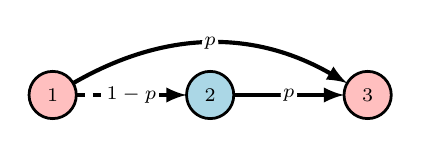
\begin{tikzpicture}[transform shape]
        \Vertex[x=-2, y=0, label=$1$, color=pink]{u1}
        \Vertex[x=0, y=0, label=$2$]{u2}
        \Vertex[x=2, y=0, label=$3$, color=pink]{u3}
        \Edge[Direct, color=black, label=$1- p$, style={dashed}](u1)(u2)
        \Edge[Direct, color=black, label=$p$, ](u2)(u3)
        \Edge[Direct, color=black, label=$p$, bend=30](u1)(u3) 
    \end{tikzpicture}} \quad
    \subfigure[Parallel Products ($d = 2$, $m = 3$).\label{fig:parallel_products}]{
    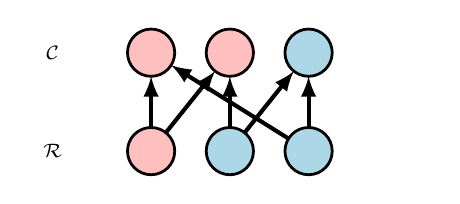
\begin{tikzpicture}[]
        \Vertex[x=-0.25,y=0,Pseudo,label={$\cR$}]{r0}
        \Vertex[x=4.25,y=0,Pseudo]{x}

        \Vertex[x=1,y=0,color=pink]{r1}
        \Vertex[x=2,y=0]{r2}
        \Vertex[x=3,y=0]{r3}

        \Vertex[x=-0.25,y=1.25,Pseudo,label={$\cC$}]{c0}

        \Vertex[x=1,y=1.25,color=pink]{c1}
        \Vertex[x=2,y=1.25,color=pink]{c2}
        \Vertex[x=3,y=1.25]{c3}  

        \Edge[color=black,Direct](r1)(c1)
        \Edge[color=black,Direct](r1)(c2)
        \Edge[color=black,Direct](r2)(c2)
        \Edge[color=black,Direct](r2)(c3)
        \Edge[color=black,Direct](r3)(c3)
        \Edge[color=black,Direct](r3)(c1)
        
    \end{tikzpicture}}
    
    %\shrink
    \caption{Production networks of \cref{sec:motivation} and \cref{sec:parallel_products}. Failures are drawn in pink color.}
    \shrink
    \label{fig:parallel_products_rdag}
\end{figure}


The first architecture we study is parallel products. Here we aim to produce $K$ complex products, which we denote by $\cC$, and each complex product requires $|\cN(i)| = m$ inputs (raw materials; source dependencies) to be produced. The set of raw materials (denoted by $\cR$) contains $|\cR| = \rho$ raw materials. We further introduce supply dependencies among the raw materials by assuming that each raw material can supply $d$ products. \cref{fig:parallel_products} shows an example of such a supply chain together with an instance of the percolation process (affected nodes are drawn in pink). Here it is interesting to study both the resilience of the whole graph, i.e., the graph with vertex set $\cC \cup \cR$, as well as the resilience of the complex products $\cC$ alone. We show that if the source dependency $m$ and the supply dependency $d$ between the products is bounded, then the production network is resilient. The resilience metric is lower-bounded by $\left ( \frac {\varepsilon} {2(d+1)m} \right )^{1/n}$ in both cases (complex products alone or together with raw materials), as the number of products goes to infinity. Moreover, if the number of inputs $m$ goes to infinity, the resilience of the whole graph goes to $0$ at rate $O \left ( e^{- \frac {1} {mn}} \right )$, and the resilience of the complex products goes to $0$ at rate $O \left ( e^{- {c^{\frac 1 m}}/{n}} \right )$ for some constant $c \in (0, 1)$. Formally, we prove the following for the resilience of the parallel products: 

% \mpcomment{Make theorems consistent and have only UB and LB there, + case when $K \to \infty$. Give intuitive explainations about the rates.}

\begin{theorem} \label{theorem:parallel_products}
    Let $\cG$ consist of $K$ parallel products and assume that these products can be produced by $|\cR| = \rho$ raw materials, and each material is used by at most $d$ products. The resilience of the complex products $\cC$ satisfies:
    $\left ( \frac {\varepsilon} {dm} + \sqrt {\frac {\log K} {2mK}} \right )^{1/n} \le R_{\cC}(\varepsilon) \le \left ( 1 - \left ( \frac {1 - \varepsilon} 2 \right )^{1/m} \right )^{1/n}$. Also, the resilience of all products satisfies: $\left ( \frac {\varepsilon} {2 (d + 1)m} + \sqrt {\frac {\log (K/2)} {2mK}} \right )^{1/n} \le R_{\cG}(\varepsilon) \le \left ( 1 - \frac {1 - \varepsilon} {2 (m + 1)} \right )^{1/n}$. Subsequently, if $\varepsilon, d$ and $m$ are independent of $K$, then then the resilience is $\Omega \left ( \left ( \frac {\varepsilon} {dm} \right )^{1/n} \right )$ as $K \to \infty$. 
\end{theorem}

\begin{proofsketch}
    For brevity, we give an analysis in expectation for $R_{\cC}(\varepsilon)$. The high-probability analysis has been deferred to Appendix \ref{app:proof:theorem:parallel_products}, where the lower bound is improved by an additive factor of $\sqrt{\frac {\log K} {2mK}}$ via Chernoff bounds. The analysis for $\cG$ is similar. To show the lower bound, we show that to have at least $\varepsilon K$ complex products fail in total, we need at least $\varepsilon K/d$ raw materials to fail. The expected number of raw materials that fail is $\rho x^n \le m K x^n$, and therefore by equating $\frac {\varepsilon K} d$ with $mKx^n$, we get the desired answer. To derive the upper bounds, we simply upper bound the expected number of surviving complex products $\ev {} {S_{\cC}} = K(1 - x^n)^m$ and apply Markov's inequality and \cref{lemma:upper_bound_resilience}.
\end{proofsketch}
\subsubsection*{Additional Results.} In Appendix \ref{app:random_trellis}, we analyze the resilience of a random width-$w$ trellis graph width $D$ tiers (and $K = wD$ nodes) where edges between subsequent tiers are generated i.i.d. with probability $p$, which can be thought of as an extension to the parallel products' architecture. In \cref{theorem:trellis_resilience}, we discover an interesting ``duality phenomenon''; i.e., when $pw \le 1$ a constant depth random trellis resilient, and when $pw \ge 1$ a constant width trellis is fragile.  

% \mar{trellis insights}
% Moreover, if $d = 1$, we can improve the lower bound of the resilience of the parallel products and show that the resilience admits an exponential improvement. The analysis is deferred in the Appendix and relies on a simple application of the Chernoff bound. 

% \begin{proposition} \label{theorem:parallel_one_resilience}
%     Let $\cG$ consist of $K$ products where each product has $m$ inputs, each input consists of $n$ suppliers, and each raw material is used by exactly $d = 1$ product. Then $R_{\cC} \ge \left ( 1 - \left  (1 - \varepsilon + \sqrt{\frac {\log K} {2K}} \right )^{1/m} \right )^{1/n}$. Subsequently, as $K \to \infty$ we have that $R_{\cG}(\varepsilon) \ge \left ( 1 - e^{-\frac {\varepsilon} {m}} \right )^{1/n}$ for $m, n, \varepsilon$ independent of $K$.
% \end{proposition}

% \begin{proofsketch}
%     The number of successfully produced complex products is a binomial variable with $K$ trials and success probability $(1 - x^n)^m$. By using standard Chernoff bounds for bounding the probability that $S_{\cC} \ge (1 - \varepsilon) K$ we get the desired result. 
% \end{proofsketch}

% \begin{proof}
%     The probability of each product being produced is $(1 - x^n)^m$, and the number of products produced follows a binomial distribution with $K$ trials and probability of success $(1 - x^n)^m$. From the Chernoff bound, we get that $\Pr [S_{\cC} \ge (1 - \varepsilon)K] \ge 1 - e^{-2K (1 - (1 - x^n)^m - \varepsilon)^2}$. We set the above probability to be $1 - 1 / K$, which yields 

%     \begin{align*}
%         x = \left ( 1 - \left  (1 - \varepsilon + \sqrt{\frac {\log K} {2K}} \right )^{1/m} \right )^{1/n}
%     \end{align*}
   
    
%     Thus we get that the resiliency of the parallel products is $R_{\cC}(\varepsilon) \ge \left ( 1 - \left  (1 - \varepsilon + \sqrt{\frac {\log K} {2K}} \right )^{1/m} \right )^{1/n}$. For $K \to \infty$, and $m, n, \varepsilon$ independent of $K$, we have that $R_{\cC}(\varepsilon) \to (1 - (1 - \varepsilon)^{1/m})^{1/n}$. Using the convexity of $e^t$ we get that as $K \to \infty$, the resilience is at least $\left ( 1 - e^{-\frac {\varepsilon} {m}} \right )^{1/n}$.
% \end{proof}

\subsection{Hierarchical Production Networks}

A supply chain can be organized hierarchically, with different levels representing different stages of the production process. The raw materials or components that go into the production of a product are at the bottom of the hierarchy, and the finished product is at the top. Each level of the hierarchy represents a stage of production where the materials or components are transformed into a more advanced or finished product \citep{elliott2022supply}. This hierarchical structure helps to visualize the flow of materials and information through the supply chain and identify potential bottlenecks or inefficiencies. Moreover, another hierarchy that is possible is producing complex products by starting from a source of raw products. In this section, we study these two hierarchies, which we call \emph{backward} and \emph{forward} (referring to the directions of the percolation with respect to the network growth), production networks visualized in \cref{fig:tree_percolation}. More specifically, we consider:
\begin{compactitem}
    \item The \emph{backward production network} (\cref{subfig:forward_backward}) at which the tree grows from the root, and then the percolation starts from the leaves and proceeds to the root. For the scope of this paper, we study backward percolation in deterministic $m$-ary trees. In \cref{sec:forward_backward_tree} we prove that, as someone would expect, such supply chains are, in fact, fragile and give lower bounds on resilience. 
    \item The \emph{forward production network} (\cref{subfig:forward_forward}) at which the tree grows from the root, and then the percolation starts from the root and proceeds to the leaves. Here, the production network is generated by a stochastic \emph{branching process}; the Galton-Watson process. In \cref{sec:forward_forward_tree}, we prove that, under specific conditions, such supply chains are fragile with a non-negative probability and are otherwise resilient.  
\end{compactitem}

\begin{figure}[t]
    \centering
    \subfigure[\label{subfig:forward_backward}]{
    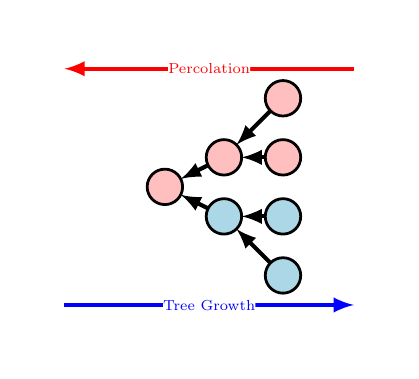
\begin{tikzpicture}[transform shape, scale=0.75]
        \Vertex[x=0, y=0, color=pink]{u1}
        \Vertex[x=1, y=0.5, color=pink]{u3}
        \Vertex[x=1, y=-0.5]{u2}
        \Vertex[x=2, y=-1.5]{u4}
        \Vertex[x=2, y=-0.5]{u5}
        \Vertex[x=2, y=0.5, color=pink]{u6}
        \Vertex[x=2, y=1.5, color=pink]{u7}

        \Edge[color=black, Direct](u2)(u1)
        \Edge[color=black, Direct](u3)(u1)
        \Edge[color=black, Direct](u4)(u2)
        \Edge[color=black, Direct](u5)(u2)
        \Edge[color=black, Direct](u6)(u3)
        \Edge[color=black, Direct](u7)(u3)

        \Vertex[x=-2, y=-2, Pseudo]{x1}
        \Vertex[x=3.5, y=-2, Pseudo]{x2}
        \Vertex[x=-2, y=2, Pseudo]{y1}
        \Vertex[x=3.5, y=2, Pseudo]{y2}

        \Edge[color=blue, Direct, label={Tree Growth}](x1)(x2)
        \Edge[color=red, Direct, label={Percolation}](y2)(y1)

        
    \end{tikzpicture}} 
    \subfigure[\label{subfig:forward_forward}]{
    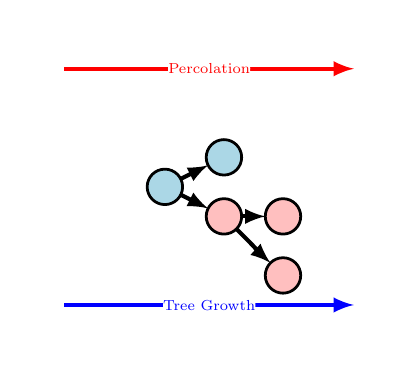
\begin{tikzpicture}[transform shape, scale=0.75]

        \Vertex[x=0, y=0]{u1}
        \Vertex[x=1, y=0.5]{u3}
        \Vertex[x=1, y=-0.5, color=pink]{u2}
        \Vertex[x=2, y=-1.5, color=pink]{u4}
        \Vertex[x=2, y=-0.5, color=pink]{u5}
        % \Vertex[x=2, y=0.5, color=pink]{u6}
        % \Vertex[x=2, y=1.5, color=pink]{u7}

        \Edge[color=black, Direct](u1)(u2)
        \Edge[color=black, Direct](u1)(u3)
        \Edge[color=black, Direct](u2)(u4)
        \Edge[color=black, Direct](u2)(u5)
        % \Edge[color=black, Direct](u3)(u6)
        % \Edge[color=black, Direct](u3)(u7)

        \Vertex[x=-2, y=-2, Pseudo]{x1}
        \Vertex[x=3.5, y=-2, Pseudo]{x2}
        \Vertex[x=-2, y=2, Pseudo]{y1}
        \Vertex[x=3.5, y=2, Pseudo]{y2}

        \Edge[color=blue, Direct, label={Tree Growth}](x1)(x2)
        \Edge[color=red, Direct, label={Percolation}](y1)(y2)
    \end{tikzpicture}}
    \subfigure[\label{fig:gw_subcritical}]{\includegraphics[width=0.3\textwidth]{figures/gw_resilience_subcritical.pdf}}
    %\shrink
    
    \caption{(a, b): Backward and Forward Networks. Node failures are drawn in pink. (c): Resilience bounds for a subcritical GW process with branching distribution as a function of $\mu$; note the decreasing trends in both upper and lower bounds, $\ev {\cG} {\overline R_{\cG}(\varepsilon)}$ and $\ev {\cG} {\underline R_{\cG}(\varepsilon)}$, with increasing $\mu$.}
    \label{fig:tree_percolation}
    \shrink
\end{figure}

In the sequel, we present the two processes and the results on $R_{\cG}(\varepsilon)$, and in \cref{sec:comparison_golub}, we compare our conclusions with the ones of \citet{elliott2022supply}.

\subsubsection{Backward Production Network} \label{sec:forward_backward_tree}

In the case of the backward production network, we consider an $m$-ary tree with height $D$ and fanout $m \ge 1$. The levels of the tree correspond to ``tiers'' with raw materials being positioned at tier $D$ and more complicated products positioned in higher tiers. Each product has $n$ potential suppliers, and each product at tier $d \in [D - 1]$ has exactly $|\cN(i)| = m$ inputs from tier $d + 1$. Tier $d = D$, which corresponds to the raw products, does not have any inputs. \cref{subfig:forward_backward} shows how the percolation process evolves in a tree with $m = 2$ and $D = 3$, where failures (drawn in pink) propagate from the two faulty raw materials up to the root.  

In addition to the power law result (\cref{theorem:power_laws}), the case of the $m$-ary tree is another example that motivates the resiliency measure $R_{\cG}(\varepsilon)$. Specifically, let's think about the probability of a catastrophic failure in a tree --- i.e., one that affects a substantial proportion of the suppliers in the production network. A raw material failing to be produced can cause its parent product not to be produced and inductively create a cascade up to the root. The complete cascade will start from the failed product at tier $D - 1$ since some products at tier $D - 1$ may be made if their corresponding raw materials are produced. However, no product can be produced from tier $D - 2$ and onward. As a result, only $o(K)$ products survive. The probability of such an event equals: 
\begin{align} \label{eq:quick}
    \Pr [S = o(K)]  \ge \Pr [\text{$\ge 1$ raw material malfunctions}] = 1 - (1 - x^n)^{m^{D - 1}} \ge 1 - e^{-x^n m^{D - 1}}. 
\end{align}
It is easy to see that if $x = \Omega \left ( \left ( {m \log K}/{K} \right )^{1/n} \right )$, then a catastrophe happens with a high probability in the tree structure, meaning that failure probabilities as small as  $\left (  {m \log K}/ {K} \right )^{1/n} + o(1)$ can cause catastrophes with probability approaching one (and therefore, the backward hierarchical production network is a fragile architecture). Therefore, it is interesting to study cases where such a scenario does not happen; on the contrary, we have many products surviving. The following Theorem formalizes lower bounds and provides an additional upper bound for the resilience of the backward production network. 

\begin{theorem} \label{theorem:tree_resilience}
    Let $\cG$ be a backward production network with fanout $m$ and depth $D$. Then, 
    \begin{align}
        \left [ 1 - \left ( 1 - \frac 1 {K} \right )^{\frac {1} {(1 - \varepsilon) K}} \right ]^{1/n} \le R_{\cG}(\varepsilon) \le \begin{cases}
            \left ( \frac {2} {K (1 - \varepsilon)}\right )^{1/n} = \left ( \frac {2} {D (1 - \varepsilon)}\right )^{1/n}, & m = 1 \\
            \left ( \frac {(1 - \varepsilon) \log m} {\log K} \right )^{1/n} \asymp \left ( \frac {(1 - \varepsilon)} {D} \right )^{1/n}, & m \ge 2. 
        \end{cases} 
    \end{align}

    Therefore, as $K \to \infty$ with $m$ finite, we have $R_{\cG}(\varepsilon) \to 0$. 
\end{theorem}

\begin{proofsketch}
    To derive the lower bound (for both $m = 1$ and $m \ge 2$), we show that if a failure happens at tier $\tau$, then all of the products up to tier $\tau$ have to be operational, which implies a lower bound on the tail probability of $S$, i.e., $\Pr [S \ge (1 - \varepsilon) K] \ge (1 - x^n)^{(1 - \varepsilon) K}$. To derive an upper bound, we show that when $m = 1$ then $\ev {} {S} \le 1 / x^n$, and when $m \ge 2$ we show (see Appendix \ref{app:upper_and_lower_bounds_tree}) that $\ev {} {S} \le KDx^n / 2$, and the rest follows by \cref{lemma:upper_bound_resilience}, and $D \ge \log K / \log m$ (for $m \ge 2$). 
\end{proofsketch}

\paragraph{Upper Bound Comparison.} Since $\varepsilon \in (0, 1)$ the above quantity behaves asymptotically as $O \left ( \left ( \frac {\log m} {\log K} \right )^{1/n} \right )$ for all values of $\varepsilon$. Therefore, the resilience goes to 0 with rate $\log K$. However, note that in \cref{eq:quick}, we showed a better rate of $O \left ( \left ( \frac {m\log K} {K} \right )^{1/n} \right )$, and therefore we state that the resilience goes to 0 with a rate of $O \left ( \left ( \frac {m\log K} {K} \right )^{1/n} \right )$ (for $m \ge 2$). 

% \mpcomment{explain which bound is better than other}

\subsubsection{Forward Production Network} \label{sec:forward_forward_tree}

We consider a random hierarchical network where the products in each level $d$ are denoted by $\cK_d$. Starting from one raw material $r$, i.e., $\cK_1 = \cR = \{ r \}$, we branch out via a Galton-Watson (GW) process such that every product $i \in \cK_d$ at level $d \ge 1$ creates $\xi_{i}^{(d)}$ supply dependencies, where $\{ \xi_{i}^{(d)} \}_{i \in \cK_d, d \ge 0}$ are generated i.i.d. from a distribution $\cD$, with mean $\ev {\cD} {\xi_{i}^{(d)}} = \mu > 0$. Subsequently, the number of products at each level obeys
\begin{align} \label{eq:gw_1}
    |\cK_{d + 1}| = \begin{cases} 
        \sum_{i \in \cK_d} \xi_i^{(d)}, & d \ge 2 \\
        1 & d = 1
    \end{cases}. 
\end{align} 

Adding the node percolation process, we start a percolation from the children of the root node $r$ and subsequently proceed to their children, and so on. The number of the surviving products $S$ in this case can be expressed as $S = \sum_{d : |\cK_d| \ge 1} \sigma_d$, where $\{ \sigma_d \}_{d \ge 0}$ follow another branching process, namely
\begin{align} \label{eq:gw_2}
    \sigma_{d + 1} = \begin{cases} 
        \sum_{1 \le i \le \sigma_d} \xi_i^{(d)} \left ( 1 - \prod_{s \in \cS(i)} Y_{is} \right ), & d \ge 2 \\
        1 - \prod_{s \in \cS(r)} Y_{rs} & d = 1
    \end{cases}. 
\end{align} 

In \cref{subfig:forward_forward}, we show such an example where failures propagate from the 


Under these scenarios, we prove the following Theorem

% \begin{lemma} \label{lemma:gw_roots}
%     For $\tau$ finite, $\frac {\one \{ \mu > 1 \}} {\log \mu} < \alpha < \frac 1 2$ , and $0 < \beta < \one \{ \mu < 1 \} + \one \{ \mu > 1 \} \frac {\log \mu - 1} {\mu} $, let 

%     \begin{align*}
%         \phi(z) & = z \frac {\mu^\tau z^\tau - 1} {\mu z - 1} - \alpha \frac {\mu^\tau - 1} {\mu - 1}, \text{ for } z \neq \frac 1 \mu, \\
%         \psi(z) & = \frac {\mu^\tau - 1} {\mu - 1} - z \frac {\mu^\tau z^\tau - 1} {\mu z - 1} - \beta, \text{ for } z \neq \frac 1 \mu.
%     \end{align*}

%     Then

%    \begin{compactenum}
%        \item If $\mu < 1$, then there exist $z_1, z_2 \in (0, 1)$ such that $\phi(z_1) = \psi(z_2) = 0$. 
%        \item If $\mu > e^2$, then there exists $z_1 \in (1/\mu, 1)$ such that $\phi(z_1) = 0$.
%        \item If $\mu > e$, then there exists $z_2 \in (1/\mu, 1)$ such that $\phi(z_2) = 0$. 
%    \end{compactenum} 

% \end{lemma} 


% \begin{proof} \textbf{Analysis for $\phi(z)$.} We do case analysis: 
%     \begin{compactitem}
%         \item If $\mu < 1$ then $\phi$ is defined everywhere in $[0, 1]$ and is also continuous. It is also easy to prove that $\phi$ is increasing in $[0, 1]$ since its the product of two non-negative increasing functions, $z$ and  $ \frac {(\mu z)^\tau - 1} {\mu z - 1} =\sum_{i = 0}^{\tau - 1} (\mu z)^i$. Moreover, note that $\phi(0) < 0$ and $\phi(1) > 0$. Therefore, there exists a unique solution $z_1 \in (0, 1)$ such that $\phi(z_1) = 0$. 
        
%         \item If $\mu > e^2$, we study $\phi$ in $(1/\mu, 1]$. Again, $\phi$ is increasing (for the same reason as above), continuous in $(1/\mu, 1]$, and has $\phi(1) > 0$. We also have that, by using L'H\^ospital's rule,

%         \begin{align*}
%             \lim_{z \to 1 / \mu} \frac {\mu^\tau z^\tau - 1 } {\mu z - 1} & = \lim_{z \to 1 / \mu} \frac {(\mu^\tau z^\tau - 1)'} {(\mu z - 1)'} = \lim_{z \to 1 / \mu} \frac {\mu^\tau \tau z^{\tau - 1}} {\mu} = \tau \implies \\
%             \lim_{z \to 1 / \mu} \phi(z) & = \frac {\tau} {\mu} - \alpha \frac {\mu^\tau - 1} {\mu - 1} < \frac {\tau (1 - \alpha \log \mu)} {\mu} < 0 \text{ for } \alpha > \frac {1} {\log \mu}.
%         \end{align*}

%         Therefore, for $\alpha \in (1/\log \mu, 1/2)$, there exists a unique solution $z_1 \in (1/\mu, 1]$ such that $\phi(z_1) = 0$. 
%     \end{compactitem}

%     % For $\tau \to \infty$, it's easy to see that $z_1 \to 1$. 

%     \textbf{Analysis for $\psi(z)$.} Note that $\psi$ is a decreasing function of $z$. We do case analysis:

%     \begin{compactitem}
%         \item If $\mu < 1$, then $\psi$ is defined everywhere in $[0, 1]$ and is continuous in $[0, 1]$. We have that $\psi(0) > 0$ and $\psi(1) < 0$ therefore there exists a unique solution $z_2$ such that $\psi(z_2) = 0$. 
%         \item If $\mu > e$, then $\psi$ is decreasing and contunuous in $(1/\mu, 1]$, with $\psi(1) < 0$. We also have that 

%         \begin{align*}
%             \lim_{z \to 1 / \mu} \psi(z) & = \frac {\mu^\tau - 1} {\mu - 1} - \frac {\tau} {\mu} - \beta > \frac {\tau (\log \mu - 1 - \mu \beta)} {\mu} > 0 \text { for } \beta < \frac {\log \mu - 1} {\mu}.
%         \end{align*}
%     \end{compactitem}

%     % For $\tau \to \infty$, it's easy to see that $z_1 \to 1$. 

% \end{proof}




\begin{theorem} \label{theorem:gw_resilience}
    Let $\cG$ be generated by a GW process where the number of children of each node is generated by a distribution $\cD$ with mean $\mu > 0$ and extinction time $\tau$. Let $G_{\cD}(\eta) = \ev {\xi \sim \cD} {e^{s\xi}}$ be the moment generating function of $\cD$, and let $\Pr [\tau < \infty]  = \eta^* = \inf \{ \eta \in [0, 1] : G_{\cD}(\eta) = \eta \}$ be the extinction probability of the GW process. Then the following are true: \emph{(i)} If $\mu < 1$, then the $\cG$ is always resilient, \emph{(ii)} If $\mu (1 - x^n) > 1$, then with probability $1 - \eta^*$, $\cG$ is fragile. 
    

    Moreover, the expected upper bound on the resilience is, for $\mu \in (0, 1) \cup (e^2, \infty)$, given by  $\ev {\cG} {\overline \cR_{\cG} (\varepsilon)} = \sum_{1 \le k < \infty} \Pr [\tau = k] \overline x(\mu, \tau, \varepsilon)$ with 
    {\footnotesize
    \begin{align}
     \overline x (\mu, \tau, \varepsilon) & = \inf \left \{ x \in \left [0, \one \{ \mu < 1 \} + \left ( 1 - \frac {1} {\mu} \right )^{1/n} \one \{ \mu > 1 \} \right ] : (1 - x^n) \frac {\mu^\tau (1 - x^n)^\tau - 1} {\mu (1 - x^n) - 1}  \le \frac {1 - \varepsilon} {2} \frac {\mu^\tau - 1} {\mu - 1} \right \}. \label{eq:ub_gw}  
    \end{align}}

    The expected lower bound on the resilience is, for $\mu \in (0, 1) \cup (e, \infty)$, given by $\ev {\cG} {\underline \cR_{\cG} (\varepsilon)} = \sum_{1 \le k < \infty} \Pr [\tau = k] \underline x(\mu, \tau, \varepsilon)$ with
    {\footnotesize
    \begin{align}
        \underline x(\mu, \tau, \varepsilon) & = \sup \left \{ x \in \left [0, \one \{ \mu < 1 \} +  \left ( 1 - \frac {1} {\mu} \right )^{1/n} \one \{ \mu > 1 \} \right ] : \frac {\mu^\tau - 1} {\mu - 1} - (1 - x^n) \frac {\mu^\tau (1 - x^n)^\tau - 1} {\mu (1 - x^n) - 1} \le \varepsilon \right \}. \label{eq:lb_gw}
    \end{align}}

\end{theorem}

\begin{proofsketch}
    If $Z_r = 0$, which happens with probability $x^n$, then the number of surviving products is $S = 0$. If $Z_r = 1$, which happens with probability $1 - x^n$, the cascade behaves as a GW process with mean $\mu_x = \mu (1 - x^n)$. Now, conditioned on the fact that $Z_r = 1$ we bound the percentage of the expected number of surviving products over the total expected number of products to devise the upper and lower bound. For the upper bound we require $\ev {\cG, x} {S} \le \frac {1 - \varepsilon} {2} \ev {\cG} {K}$, and for the lower bound we require $\ev {\cG, x} {F} = \ev {\cG} {K} - \ev {\cG, x} {S} \le \varepsilon$. We prove that if the process takes infinite time to terminate, then the only possible solution is $x = 0$ which makes the supply chain fragile. In all of the other cases, we study the existence of an upper and a lower bound to the resilience by solving two inequalities, whose roots are studied in (the auxiliary) \cref{lemma:gw_roots}. 
\end{proofsketch}

Applying \cref{theorem:gw_resilience} for the case where $\cD$ is a point-mass function that equals $\mu$ with probability $1$, yields the following corollary for deterministic structures (when $\mu \in \mathbb N^*$ these are trees).

\begin{corollary}
    Let $\cD$ have $\Pr_{\xi \sim \cD} [\xi = \mu] = 1$ for $\mu > 1$. Then $\cG$ is 
always fragile.
\end{corollary}


% \mpcomment{put corrolary there for deterministic tree}

For the subcritical regime, we plot the expected resilience bounds in \cref{fig:gw_subcritical} for a subcritical GW process with branching distribution $\cD = \mathsf{Bin}(k, p \in (0, 1 / k))$, as a function of $\mu = k p$. 

% \begin{figure}
%     \centering
%     \includegraphics[width=0.5\textwidth]{figures/gw_resilience_subcritical.pdf}
%     \shrink
%     \caption{Resilience bounds for a subcritical GW process with branching distribution as a function of $\mu$; note the decreasing trends in $\ev {\cG} {\overline R_{\cG}(\varepsilon)}$ and $\ev {\cG} {\underline R_{\cG}(\varepsilon)}$ with increasing $\mu$.}
%     \shrink
%     \label{fig:gw_subcritical}
% \end{figure}

% \mpcomment{replace complexity with dependency}

\subsubsection{Comparison with the results of \texorpdfstring{\citet{elliott2022supply}}{elliott2022supply}.}\label{sec:comparison_golub} The work of \citet{elliott2022supply} considers a hierarchical supply network similar to the one presented in \cref{sec:forward_backward_tree} -- though by assuming a different percolation process. In Section II of their paper they observe that as the interdependency increases then their reliability metric decreases, and as the number of suppliers increases then the reliability increases. This is in agreement with the lower bound presented in \cref{theorem:tree_resilience} for the backward production network which increases as $n$ increases and decreases as $m$ increases, probability that there's at least a raw material failure (\cref{eq:quick}) increases. Moreover, in their paper, if the shocks are below a value then for large depths, the reliability goes to zero, which is conceptually in agreement with the upper bounds presented in \cref{theorem:tree_resilience}, which go to zero as $D$ grows. Finally, for the forward production network -- which is not studied by \citet{elliott2022supply} -- we again get a result that is in agreement with their results, since as the average interdependency $\mu$ increases we observe that the upper and lower bounds in the resilience decrease, as empirically shown in \cref{fig:gw_subcritical}.  

\subsection{Techniques for General Production Networks} \label{sec:general_supply_chains}

% \mpcomment{move discussion about circular economies to the discussion section, talk only about cycles in supply chains}

So far, we have focused our attention on simple structures where we can find analytical expressions for $\ev {} {F}$, and, subsequently, by bounding $\ev {} {F}$ we can determine the upper and / or lower bounds for $R_{\cG}(\varepsilon)$. However, in more general cases, $\cG$ may have a more complicated structure for which we want to calculate the resilience, and in general, $\ev {} {F}$ is \#P-hard to compute; cf. \citep{chen2010scalable}.%, and in general, any sampling-based algorithm has complexity at least $\Omega (K + M)$ \citep{borgs2014maximizing}. 
Moreover, it is certainly possible for a production network to have cycles, e.g., when complex products are used in the production of simpler products. It is also possible that production networks have cycles that represent recycling or other forms of circular flows of materials or resources in modern economies; cf. circular economies \citep{geissdoerfer2017circular}. In this section, we offer techniques to address the following questions for general network topologies:  
% such as in the case of circular economies \citep{geissdoerfer2017circular,kirchherr2017conceptualizing}. In some cases, production networks can have cycles, which can represent recycling or other forms of circular flows of materials or resources. 
\begin{compactenum}
\item[\emph{Question 1.}] \emph{How do we efficiently calculate the cascade size $F$?}
\item[\emph{Question 2.}] \emph{How do we identify network vulnerabilities in the failure of their most critical nodes?}
\item[\emph{Question 3.}] \emph{How can we design interventions to minimize the (expected) size of failure cascades?}
\end{compactenum}

As expected, production networks are most vulnerable to failure of their most ``central'' nodes, to which many of their products have (potentially higher order) connections. In fact, we can identify such nodes using their Katz centrality \citep{katz1953new}, which arises naturally under certain assumptions in our model. Moreover, efficient network protection can be achieved to minimize the size of cascading failures (in part) by protecting the most central nodes, which we formulate in \cref{sec:interventions}.

A surprising way to identify such nodes involves extending the percolation process to allow link failures, creating a noisy version of the node percolation process introduced in \cref{sec:node_percolation}. More specifically, for each edge $(i, j) \in \cE(\cG)$ of the production network, we flip a coin of bias $y \in (0, 1]$, independently of the other edges and suppliers, and decide to keep the edge with probability $y$. Model-wise, this corresponds to firms holding inventories and, therefore, if a product $i$ has enough inventory from its input product $j$, then it is likely to discard its network dependencies with probability $1 - y$. 

This creates a subsampled graph $\cG_y \subseteq \cG$, which, under reasonable assumptions for $x$ and $y$, can be used to identify vulnerabilities of the network to products whose failure is likely to cause the largest cascading failures. The above process can also be viewed as a \emph{joint percolation} on both nodes and edges or a node percolation on the noisy subnetwork $\cG_y$, where in order for a product to function, on average it only needs a $y$-fraction of its inputs to operate. We define $R_{\cG}(\varepsilon; y)$ as resilience assuming randomness in the sampling $\cG_y$, such that $R_{\cG}(\varepsilon) = R_{\cG}(\varepsilon; y = 1)$. Moreover, we define $F_y$ as the size of the cascade in $\cG_y$ and $F$ as the size of the cascade when $y = 1$. A simple coupling argument similar to \cref{lemma:upper_bound_resilience} for $0 < y_1 \le y_2 < 1$ shows that survivals in $\cG_{y_1}$ are greater than in $\cG_{y_2}$: 

\begin{proposition} \label{prop:rel_resilience}
    For any $0 < y_1 \le y_2 \le 1$, we have $R_{\cG} (\varepsilon; y_1) \ge R_\cG(\varepsilon; y_2)$. Subsequently, $R_\cG (\varepsilon; y) \ge R_{\cG}(\varepsilon)$ for all $y \in (0, 1]$. 
\end{proposition}

 In the following, we answer the above questions and provide a systematic way to treat general graphs that undergo a joint percolation process. More specifically, we systematically bound the expected number of failures and subsequently derive bounds for the resilience metric. Finally, we show that our analysis has deep connections to financial networks. To put our analysis into a mathematical framework, Markov's inequality states $\Pr [F_y \ge \varepsilon K] \le {\ev {} {F_y}} /{\varepsilon K}$. This together with \Cref{prop:rel_resilience} allows us to have an upper bound on resilience by limiting the failure of at least $\varepsilon K$ products which requires an upper bound on $\ev {} {F_y} = \sum_{i \in \cK} \Pr [Z_i = 0]$ following Markov's inequality; recalling notation of \Cref{eq:dynamics}, $Z_i$ is an indicator variable for the failure of product $i$. 

To connect the approximation of $\ev {} {F_y}$ with linear programming, we define the following optimization problem and its dual, with optimal solutions $\beta_{\cG}^*(u; y)$ and $\gamma_{\cG}^*(u; y)$, which are parametrized by a shock vector $u \in [\zero, \one] := [0,1]^{K}$: 

\begin{align}
	p_\cG^*(u; y) & = \max_{\beta \in [\zero, \one]}  \one^T \beta \quad &
	\text{s.t.} \quad & \beta \le y A^T \beta + u, \label{eq:upper_bound_lp} \\
        d_{\cG}^*(u; y) & = \min_{\gamma, \theta \ge \zero}  u^T \gamma + \one^T \theta \quad & \text{s.t.}  \quad  & (I - yA) \gamma  + \theta \ge \one. \nonumber%\label{eq:upper_bound_lp_dual} 
\end{align}

 When the context is evident, we skip the arguments and simply write $p^*, d^*, \beta^*$ and $\gamma^*$. The following theorem gives a way to characterize an upper bound on $\ev {} {F_y}$ as the solution to a linear program (proof in Appendix \ref{app:proof:theorem:general_ub}).


\begin{theorem} \label{theorem:general_ub}
    Let $\cG$ be a production network that undergoes a joint percolation process with the probability of supplier failure $x$ and the probability of survival of edges $y$. If $p^*$ is the optimal value of the primal problem in \cref{eq:upper_bound_lp} for $u = \one x^n$, then, for $y = \varrho / m$ and $\varrho \in (0, 1)$, we have $\ev {} {F_y} \le p^* \le \left (1 + \varrho + O((\varrho)^2) \right ) \ev {} {F_y}$. The solution to LP can be found as the unique fixed point $\beta^*$ of the contraction $\Phi(\beta) = \one \wedge (y A^T \beta + x^n \one)$.
\end{theorem}

The above theorem provides an algorithm to find $\beta^*$ by solving the fixed point problem, i.e., if $\beta^{(t)}$ corresponds to the failure probabilities in iteration $t$, then $\beta^*$ can be found using the following iteration which corresponds to a contraction map (since $y < 1/m$):
\begin{align}
    \beta^{(t)} = \one \wedge \left (yA^T \beta^{(t - 1)} + x^n \one \right ). \label{eq:contarction_iteration}
\end{align}

% \begin{proofsketch}
%     The proof uses a union bound on $\beta_i = \Pr [Z_i = 0]$ for every $i \in \cK$ and maximizes $\sum_{i \in \cK} \Pr [Z_i = 0]$ under the union bound constraint and the fact that $\{ \Pr [Z_i = 0] \}_{i \in \cK}$ are valid probabilities. Moreover, due to optimality $p^* \ge \ev {} {F_y}$. To get the upper bound, note that if $\beta^*$ is an optimal solution, then the union bound constraint implies that $(1 - my) \sum_{i = 1}^K \beta_i^* \le Kx^n \le \ev {} {F_y}$. Using the fact that $\frac {1} {1 - my} = 1 + my + O((my)^2)$ we get the right hand side. The final part of the proof applies \citep[Lemma 4]{eisenberg2001systemic}. 
% \end{proofsketch}

To obtain a solution with precision $\eta$, we need to iterate \cref{eq:contarction_iteration} $\log(2K/\eta) / \log (1 / \varrho)$ times,  where $\varrho < 1$ is the Lipschitz constant for the contraction map and $2K$ bounds the $L_1$ norm of the initial condition.  This algorithm has a runtime of $O \left ( \frac {(K + M)\log (K / \eta)} {\log (1 / \varrho)} \right ) = \tilde O(K + M)$ to yield a solution that is close to $\beta^*$ by some accuracy $\eta$, and subsequently is a $1 + \eta + \varrho + O(\varrho^2)$ approximation of the cascade size. The runtime matches the lower bound (up to logarithmic factors) $\Omega(K + M)$ of the influence maximization problem as shown in \cite{borgs2014maximizing}. We also show that the following approximation bounds hold for $F_y$ and also that $\ev {} {F_y}$ can never give a better approximation than $3/4 + o(1)$ -- the proof is in Appendix \ref{app:proof:theorem:Fy_approximation}. 

 \begin{theorem} \label{theorem:Fy_approximation}
    For $y < 1 / m$, we have $\ev {} {F_y} \ge \frac {\ev {} {F} - Kq} {1 - q}$ where $q = (1 - (1 - x^n(1 - y))^m$. Moreover, $\ev {} {F_y} \le \left ( \frac {3} {4} + o(1)  \right ) \ev {} {F}$.
 \end{theorem}


% \textcolor{red}{Combining \cref{theorem:general_ub,theorem:Fy_approximation}, we get that the LP yields a $3/4 + o(1)$ approximation to $\ev {} {F}$ for $y < 1/m$.} 
\cref{theorem:general_ub} shows that there is a systematic way of bounding $\ev {} {F}$ and $\ev {} {F_y}$ via the solution of a linear program or a fixed-point equation (if the edge survival probability is less than $1/{m}$). It is surprising to note that an elegant upper bound on the expected number of failures becomes possible by introducing sampling at the edge level which reduces network dependencies. Moreover, if we want to maximize a weighted cascade, namely the objective function is $\pi^T \beta$ for some vector $\pi \ge \zero$ instead of $\one^T \beta$, then the corresponding dual program, corresponds to the systemic risk measure \citep[Example 7]{chen2013axiomatic}: $$\Lambda_{\cG}(\pi; x) = \min_{\gamma, \theta \ge \zero} x^n \one^T \gamma + \one^T \theta \quad \text{s.t.} \quad (I - yA)\gamma + \theta \ge \pi.$$
 
% \begin{algorithm}[t]
%     \scriptsize
%     \captionof{algorithm}{Solution to \cref{eq:upper_bound_lp} for DAGs\label{alg:dag_upper_bound}}
%     \begin{flushleft}
%     \textbf{Input:} DAG $\cG$, node percolation probability $x$, number of suppliers $n$, edge sampling probability $y$. \\
%     \textbf{Output:} The solution ${\beta^*}$ to the linear program in \cref{theorem:general_ub} ---  \cref{eq:upper_bound_lp}. 
%     \medskip
%     \begin{compactenum}
%         \item Use depth-first search to create a topological ordering of DAG $\cG$, $\pi : \cK \to \cK$, and let ${\beta^*}_{\pi(1)} = x^n$
%         \item For $2 \le i \le K$, set ${\beta^*}_{\pi(i)} = \min \left \{ 1, y \sum_{j \in \cN(\pi(i))} \beta^*_j + x^n \right \}$
%     \end{compactenum}
%     \end{flushleft}
% \end{algorithm}




% However, \cref{theorem:general_ub} gives a polynomial time algorithm to compute an \emph{upper bound} on $\ev {\cG, y, x} {F}$ by solving the aforementioned LP. \cref{alg:dag_upper_bound} solves this LP when $\cG$ is a DAG in $O(K + |\cE(\cG)|)$ time. When we allow cycles in $\cG$, the calculation becomes more complicated, and \cref{alg:dag_upper_bound} does not produce a valid solution, and we instead have to rely on solving the LP. 



After defining $p^*_{\cG}$ and its dual $d^*_{\cG}$, the next question is how they are related to resilience. In the following (proved in Appendix \ref{app:proof:theorem:lp_duality_resilience}), we show that we can bound the resilience using the sum of the Katz centralities $\beta_\cG^\katz(y) = (I - yA^T)^{-1} \one$ in $\cG$.

\begin{theorem} \label{theorem:lp_duality_resilience}
    If $y < 1/m$, the resilience $R_{\cG}(\varepsilon; y)$ satisfies $R_{\cG}(\varepsilon; y)  \ge \left (\frac {\varepsilon} {\one^T \beta_{\cG}^\katz (y)} \right )^{1/ n}$.
\end{theorem}

% In the case of DAGs, we can get a special lower bound for $R_{\cG}(\varepsilon; y)$, in the large-shock regime for edges, i.e., when edges fail with high probability $1-y$. 

% \begin{proposition} \label{prop:dag_lb_sparse}
%     Let $\cG$ be a DAG, and consider the joint percolation process with node percolation probability $x \in (0, 1)$, and edge survival probability $y \in (0, 1)$. Then $$R_{\cG}(\varepsilon; y) \ge \left ( \frac {\varepsilon y} {e^{Ky}} \right )^{1/n}.$$ 
    
%     When $y = \frac 1 K$, the lower bound on the resilience is maximized and equals $\left ( \frac {\varepsilon} {e K} \right )^{1/n}$.
% \end{proposition}

% \begin{proofsketch}
%     We consider a topological order of the DAG and prove that the solution $\beta^*$ to the linear program of \cref{theorem:general_ub} --- \cref{eq:upper_bound_lp} --- satisfies $\beta_i^* \le (1 + y)^{i - 1} x^n$ for all $i \in \cK$. Therefore, we can prove that the expected number of failures is at most ${x^n e^{K y}}/ {y}$ which is minimized for $y = 1/K$, yielding the maximized lower bound on  $R_{\cG}(\varepsilon)$. 
% \end{proofsketch}

% An immediate consequence of \cref{{prop:dag_lb_sparse}} is that whenever there is an over-diversification of suppliers, i.e., $n \ge Ky$, then every DAG is resilient --- in agreement with the results of \citet{elliott2022supply}. This idea of maximizing $\ev {} {F}$ has its roots in financial networks, specifically the Eisenberg-Noe model of financial contagion among agents with assets and liabilities \citep{eisenberg2001systemic, glasserman2015likely}. Similar connections between the Eisenberg-Noe clearing problem and network centrality have been made by \citet{siebenbrunner2018clearing,bartesaghi2020risk} and references therein. 

% Moreover, the solution to \cref{eq:upper_bound_lp} gives a measure of \emph{``vulnerability''} of each node, i.e., how likely they are to be affected by cascading failures. In case of DAGs, we can relate this ranking of the node vulnerabilities to their topological ordering as follows:

% \begin{corollary}
%     If $\cG$ is a DAG, $\pi : \cK \to \cK$ is a topological ordering of the nodes in $\cG$, and $\beta^*$ is the solution to the linear program in \cref{eq:upper_bound_lp}, then $\beta^*_{\pi(i)} \le \beta^*_{\pi(j)}$ for all $1 \le i \le j \le K$. 
% \end{corollary}

% The preceding corollary, which is a direct consequence of \cref{theorem:general_ub} and \cref{alg:dag_upper_bound}, states that when $\cG$ is a DAG, the least vulnerable nodes are the raw materials that precede more complex products in their topological ordering. On the other hand, the failure of raw materials in a DAG will cause large cascading failures, affecting all the complex products that succeed the raw materials in their topological ordering. Hence, to prevent large cascading failures, it seems intuitive to intervene to protect nodes that rank highest in the reversed graph. Our results in the next section formalize this intuition, giving an explicit solution for optimal interventions in terms of the Katz centrality of the reversed graph (\cref{prop:intervention}).    

So far, we have focused on the regimes where $y < 1/m$. A reasonable question to ask here is whether the LP bounds are a good approximation of $\ev {} {F_y}$ for $y > 1/m$. Unfortunately, the answer is negative as we show in Appendix \ref{app:innaproximability} as we can find families of graphs such that the gap between the LP and $\ev {} {F_y}$ is at least $K / 8$.



%  .... This gives a clear way to design interventions on a DAG, which would involve intervening on $\pi(1), \dots, \pi(T)$

% \subsection{Relationship to Input-Output Matrices}

% \mpcomment{talk about Leonfieff inverse, input output matrices, etc. see the production networks primer review for ideas}


% \begin{figure}[t]
%     \centering
%     \begin{tikzpicture}[transform shape]
%         \Vertex[x=-1, y=0, label=$1$]{u1}
%         \Vertex[x=1, y=0, label=$2$]{u2}
%         \Vertex[x=0, y=1, label=$3$]{u3}
%         \Edge[Direct, color=black](u2)(u1)
%         \Edge[Direct, color=black](u2)(u3)
%         \Edge[Direct, color=black](u3)(u1)
        
%     \end{tikzpicture}
    
    
%     \caption{Example for \cref{theorem:general_ub}. The optimization of \cref{theorem:general_ub} yields $\beta = ((1 + y)^2 x^n, x^n, (1 + y) x^n)$ and a bound $\ev {} {F} \le \frac {(1 + y)^3 x^n} {y}$.}
%     \label{fig:optimization2}
% \end{figure}

\subsection{Intervention Design} \label{sec:interventions}

% Safeguarding supply chains is an ever-important issue in supply-chain management. Many potential risks can disrupt the supply chain and impact a business's operations and bottom line. These risks can include natural disasters, transportation issues, supplier bankruptcy, cyber-attacks, geopolitical turmoils, etc. It is important for suppliers to have contingency plans to address potential supply chain disruptions and minimize their impact. 


In our model, we build intuition behind designing interventions to protect the supply chain. Our problem involves a global planner that can treat a maximum of $B$ products in the network. Regulators aim to minimize failures, which can be achieved in many ways, such as diversifying the supplier base, building inventory buffers, and implementing robust risk management and monitoring systems. In mathematical terms, since each product can be produced if it has at least one functional supplier, this is equivalent to selecting a maximum of $B$ products in which to intervene. The decision variables are set to $t_i \in \{ 0, 1 \}, i \in \cK$, corresponding to the subset $T \subseteq \cK$ of treated products). The probability of failure of every product is then given by $(x(1 - t_i))^n = x^n (1 - t_i)$. Abusing notation, we define $p_{\cG}^*(T; y)$ (resp. $d_{\cG}^*(T; y)$) as the value of $p_{\cG}^*(u; y)$ (resp. $d_{\cG}^*(u; y)$) where $u_i = 0$ for every $i \in T$ and with $F(T)$ (resp. $F_y(T)$) to be the cascade size (resp. cascade size on the subsampled graph) after treating the products in $T$. A candidate problem for the planner in this case is 

\begin{align} \label{eq:optimal_interventions_opt}
    \min_{T \subseteq \cK : |T| = B} p_{\cG}^*(T; y) = \min_{T \subseteq \cK : |T| = B} d_{\cG}^*(T; y)
\end{align}

The function $p_{\cG}^*(T; y)$ is increasing and submodular as a direct consequence of \cite[Online Appendix, Proposition A.7]{banerjee2022pricing}. Therefore, the intervention problem focuses on minimizing a monotone, increasing sub-modular function. This problem can be solved in polynomial time by relying on the Lov\'asz extension of $p_{\cG}^*(T; y)$. For small shocks, we can solve the intervention problem analytically. Specifically, if $0 < y < \frac 1 {\max \{m, \mu \}}$ and $0 < x < (1 - y \max \{ m, \mu \})^{1/n}$, then the optimal solution of the maximization LP in \cref{eq:optimal_interventions_opt} (since the constraint that corresponds to the network and individual effects holds with equality) is $\hat \beta (T) = x^n (I - yA^T)^{-1} \one_{\cK \setminus T}$ where $\one_{\cK \setminus T}$ is the indicator vector of $\cK \setminus T$. This yields the following proposition (proved in Appendix \ref{app:prop:intervention}).

\begin{proposition} \label{prop:intervention}
    Let $0 < y < \frac 1 {\max \{m, \mu \}}$, $0 < x < (1 - y \max \{m, \mu \})^{1/n}$. Let $\cG^R$ be the graph where the direction of the edges in $\cG$ is reversed, and consider $\gamma_{\cG}^\katz(y) = (I - yA)^{-1} \one$, the Katz centrality of $\cG^R$. Let $\pi : \cK \to \cK$ be a decreasing order on the entries of $\gamma_{\cG}^\katz(y)$. Then, the optimal policy $\hat t$ sets $\hat t_{\pi(i)} = 1$ for $i \in [B]$ and sets it to zero otherwise.
\end{proposition}

So, we can think of the ``riskiest'' products to be the ones with a high Katz centrality in $\cG^R$  --- the reversed graph representing the sourcing relationships between products. This agrees with our intuition about DAGs, which says to intervene starting from the raw materials and progressing in the topological order of the DAG until the budget is exhausted. 

% \mpedit{In the more general case when $y$ is large and $x$ has arbitrary values, it is a direct consequence of the results of \citep{papachristou2024optimal,banerjee2022pricing} that $p_{\cG}^*(u; y)$ is $K$-increasing and submodular in $u$, and that the intervention problem can be equivalently phrased as identifying $K - T$ products to place on the failures. This problem is NP-Hard by a reduction from the 3-Set-Cover problem (see also \cref{theorem:resilience_deterministic_hardness} later in the paper), which yields an $(1 - 1/e)$-approximation algorithm. 

% \begin{proposition} \label{prop:intervention_general}
%     Let $\cG$ be a graph of maximum outdegree $m \ge 1$, let $\cG^R$ be the graph where the direction of edges in $\cG$ are reversed, and let $\mu$ be the maximum outdegree of $\cG^R$. Let $ y \ge \frac 1 {\min \{ m, \mu \}}$. Then, the greedy hill-climbing algorithm yields a policy $t^{\mathsf{sol}}$ such that $p_{\cG}^*((\one - t^{\mathsf{sol}}) x^n; y) \ge \left ( 1 - \frac 1 e \right ) p_\cG^*((\one - t^{\mathsf{opt}})x^n; y)$. 
% \end{proposition}}


\subsection{The Risk Exposure Index} \label{sec:rei}

Our metric has connections to important metrics already present in the supply chain literature \citep{levi2016identifying,simchi2014superstorms,ham2022companies}, such as the Risk Exposure Index (REI). To define REI, suppose that a product in the production network is disrupted by an infinitesimal shock, assuming the same responses from the other nodes. In our case, this corresponds to a change in the probability of shock of the product $i$ from $x$ to $x + \delta$ and its impact on the size of cascading failures, which corresponds to the potential impact $\potentialimpact(i)$. Since it is difficult to quantify an exact formula for the change of $\ev {} {F}$, we will instead focus on the change in $\ev {} {F_y}$ given by \cref{eq:upper_bound_lp}. Specifically, the potential impact for a node is defined as 

{\small
\begin{align} \label{eq:potential_impact}
    \potentialimpact_i (x; y) & = \lim_{\delta \to 0} \frac {p_\cG^*\left ((x^n, \dots, (x + \delta)^n, \dots, x^n)^T; y\right ) - p_\cG^* \left ( (x^n, \dots, x^n, \dots, x^n )^T; y\right )} {\delta} = \left (  n x^{n - 1} \right ) \cdot \frac {\partial \beta_i^*(u; y)} {\partial u_i} \bigg |_{u_i = x^n}.
\end{align}}

Subsequently, the Risk Exposure Index of $\cG$ (REI, \cite{levi2016identifying}) is given as the worst possible magnitude of $\potentialimpact_i(x; y)$, i.e.,

\begin{align} \label{eq:rei}
    \rei_{\cG}(x; y) = \max_{i \in \cK} |\potentialimpact_i(x; y)| = n x^{n - 1} \left \| \frac {\partial \beta^*} {\partial u} \bigg |_{u = \one x^n} \right \|_{\infty}.
\end{align}

We give the following Theorem to characterize the REI:

\begin{theorem} \label{theorem:marginal_rei}
    Consider an optimal solution $\beta^\star$ of \cref{eq:upper_bound_lp}. Let $\cK^+  = \left \{ i \in [K]: \beta_i^* = 1, \beta_i^* \le y \sum_{j \sim i} \beta_j^* + x^n \right \}, \cK^- = \left \{ i \in [K] : \beta_i^* < 1, \beta_i^* =  y \sum_{j \sim i} \beta_j^* + x^n \right \}, \cK^0 = \left \{ i \in [K] : \beta_i^* =1 =  y \sum_{j \sim i} \beta_j^* + x^n \right \}$ be a partition of the products $\cK$. Let $\cB^+ = \cK^- \cup \left \{ K + j : j \in \cV^+ \cup \cV^0 \right \}, \cB^- = \cK^+ \cup \left \{ K + j : j \in \cV^- \cup \cV^0 \right \} $ be the bases of the equivalent LP with variable $s$, that is, $\max_{\beta, s \ge \zero} \; \one^T \beta$ subject to $(I - yA^T) \beta + s = \one x^n$ and $\beta \le \one$. If $B^+$ and $B^-$ are the matrices formed by the columns of $\begin{pmatrix} I - yA^T & I\end{pmatrix}$ corresponding to $\cB^+$ and $\cB^-$, and 

    {\small
    \begin{align*} 
    \potentialimpact^{+}_i (x; y) =  \left (  n x^{n - 1} \right ) \cdot \frac {\partial^+ \beta_i^*(u; y)} {\partial u_i} \bigg |_{u_i = x^n}, \rei^{+}_{\cG}(x) = \max_{i \in [K]} |\potentialimpact^{+}_i(x; y)|, \\ \potentialimpact^{-}_i (x; y) =  \left (  n x^{n - 1} \right ) \cdot \frac {\partial^- \beta_i^*(u; y)} {\partial u_i} \bigg |_{u_i = x^n}, \rei^{-}_{\cG}(x; y) = \max_{i \in [K]} |\potentialimpact^{-}_i(x; y)|,
    \end{align*}}
     
    then $\rei^{+}_\cG(x; y) = n x^{n - 1} \left \| \begin{pmatrix} I & O \end{pmatrix}_{\cdot, \cB^+} \left ( B^+ \right )^{-1} \right \|_{\infty}$ and $\rei^{-}_\cG(x; y) = n x^{n - 1} \left \| \begin{pmatrix} I & O \end{pmatrix}_{\cdot, \cB^-} \left ( B^- \right )^{-1} \right \|_{\infty}$. 

    Moreover, if there are no borderline nodes (i.e., $\cK^0 = \emptyset$), then $\cB^+ = \cB^- = \cB$, $B^+ = B^- = B$, and subsequently $ \rei_\cG(x; y) = n x^{n - 1} \left \| \begin{pmatrix} I & O \end{pmatrix}_{\cdot, \cB} \left ( B \right )^{-1} \right \|_{\infty}$.   
\end{theorem}

\cref{theorem:marginal_rei} is a direct consequence of applying Proposition 1 of \cite{liu2010sensitivity}. We can also show that when firms hold large enough inventory ($y < 1/m$) and the shocks are sufficiently small the REI is proportional to the node with the highest Katz centrality in $\cG^R$. 

\begin{corollary} \label{collorary:rei_katz}
    If $y < 1/ m$, and $x < (1 - my)^{1/n}$,  then $\mathrm {REI}_\cG(x; y) = n x^{n - 1} \| \gamma_\cG^\katz(y) \|_\infty.$
\end{corollary}



\subsection{Resilience of Empirical Production Networks} \label{sec:experiments}

% \begin{figure}
%     \centering
%     \includegraphics[width=0.5\textwidth]{figures/statistics.pdf}
%     \caption{Network statistics for the three networks studied in \citet{willems2008data}}
%     \label{fig:msom_willems_statistics}
% \end{figure}

With the definition of resilience and the theoretical results developed in the previous sections, we study the resilience of production networks in practice. We examine the resilience of networks contained in the following two data sets of production networks (\cref{tab:statistics-willems,tab:statistics-world}):  

\begin{compactenum}
    \item \emph{Multi-echelon Supply-chain Networks} from \citet{willems2008data}. The dataset contains 38 different multi-echelon (see also \cref{fig:supply_chain}) supply chain networks, from which we select three networks to run simulations on.  Similar supply chain networks have been used in prior literature, see, e.g., \citet{blaettchen2021traceability} and \citet{perera2017network}. 
    \item \emph{Country Economy Production Networks} derived from \emph{World Input-Output Tables} taken from the World Input-Output Database \citep{timmer2015illustrated}. We focus on the economies of six countries in 2014: the USA, Japan, China, Great Britain, Indonesia, and India. We consider any non-zero amount cell at the input-output tables as an edge between two industries in a country. For space considerations, the results have been deferred to Appendix \ref{app:experiments_addendum}. 
\end{compactenum}

% \begin{table}[H]
%     \footnotesize
%     \centering
%     \begin{tabular}{lllllll}
%     \toprule
%          Network ID  & Size ($K$) & Avg. Degree & Density & Min/Max In-degree & Min/Max Out-degree  & AUC  \\
%     \midrule 
%     \multicolumn{7}{c}{Networks from \citet{willems2008data}} \\
%     \midrule
%          \#10 & 58 & 3.03 & 0.053 & 0 -- 27 & 0 -- 13  & 0.136 \\
%          \#20 & 156 & 1.08 & 0.006 & 0 -- 29 & 0 -- 3  & 0.117 \\
%          \#30 & 626 & 1.00 & 0.001 & 0 -- 2 & 0 -- 48  & 0.357 \\ 
%     \midrule
%     \multicolumn{7}{c}{World I-O Tables} \\
%     \midrule
%          USA & 55 & 54.00 & 1.000 & 54 & 54 & 0.052 \\
%          Japan & 56 & 45.33 & 0.824 & 0 -- 50 & 0 -- 50  & 0.058 \\
%          G. Britain & 56 & 52.05 & 0.946 & 0 -- 54 & 0 -- 54  & 0.052  \\
%          China & 56 & 37.89 & 0.688 & 0 -- 46 & 0 -- 46  & 0.078 \\
%          Indonesia & 56 & 35.75 & 0.65 & 0 -- 46 & 0 -- 46  & 0.078 \\
%          India & 56 & 29.57 & 0.537 & 0 -- 41 & 0 -- 43 & 0.095 \\
%     \bottomrule
%     \end{tabular}
%     \caption{Network Statistics and AUC. The edge density is computed as $\frac {|\cE(\cG)|} {K^2 - K}$.}
%     \label{tab:statistics}
% \end{table}


\begin{table}[!htbp] \centering
\scriptsize
\begin{tabular}{@{\extracolsep{5pt}}lc}
\\[-1.8ex]\hline
\hline \\[-1.8ex]
& \multicolumn{1}{c}{\textit{Dependent variable: log-$\Ravg {\cG} (y)$}} \
\cr \cline{2-2}
\hline \\[-1.8ex]
 const & -1.757$^{***}$ (0.045) \\
 log-$K$ & 0.146$^{***}$ (0.012) \\
 log-$r$ & -0.029$^{***}$ (0.010) \\
\hline \\[-1.8ex]
 Observations & 34 \\
 $R^2$ & 0.871 \\
 Adjusted $R^2$ & 0.862 \\
 Residual Std. Error & 0.067 ($df=31$) \\
 $F$ Statistic & 104.385$^{***}$ ($df=2; 31$) \\
\hline
\hline \\[-1.8ex]
\textit{Note:} & \multicolumn{1}{r}{$^{*}p<0.1; ^{**}p<0.05; ^{***}p<0.01$} \\
\hline \\
\end{tabular}
\caption{Relation between the $\Ravg {\cG} (y)$, $K$ and $r$ for the multi-echelon networks of \cite{willems2008data}. For each network, we set $y = 1 / (m + 10^{-5})$.}
\label{tab:resilience_auc}
\shrink
\end{table}


\xpar{Resilience metrics} First, we study the resilience of the above networks as a function of $\varepsilon$ for $\varepsilon$ ranging from 0 to 1 numerically. To achieve this, we run $1000$ Monte Carlo (MC) simulations where we sample the (spontaneous) state of $n$  suppliers and then propagate the state of each product to the adjacent ones, based on \cref{eq:dynamics}. To calculate resilience, we estimate the probability $\Pr [S \ge (1 - \varepsilon) K]$ for various values of $x \in (0, 1)$ with MC simulation and find the maximum value of $x$ for which the estimate is at least $1 - 1 / K$. We plot the estimated resilience $\hat R_{\cG}(\varepsilon)$ as a function of $\varepsilon$. and present the results in \cref{subfig:willems_resilience,subfig:world_io_tables_resilience}. As an additional resilience metric that's independent of $\varepsilon$, we also report the average resilience $\Ravgsamp {\cG}(y) = \int_0^1 \hat R_{\cG}(\varepsilon; y) d \varepsilon$.  

Furthermore, we perform a regression to relate $\Ravgsamp {\cG}(y)$  with the number of raw products ($r$) and the size of the network ($K$), and report the results in \cref{tab:resilience_auc}. We find that $\Ravgsamp {\cG} (y)$ increases in $K$ ($p < 0.01$) and decreases with $r$ ($p < 0.01$). This agrees with our theoretical results (e.g., \Cref{theorem:resilience_graph_statistics}) which highlight that networks with more raw products have lower resilience.

\xpar{Optimal interventions} To study the effect of targeted interventions in real-world supply chain networks, we apply the results of \cref{prop:intervention} for the networks from the two datasets. More specifically, for a value of $y = \frac {1} {10^{-5} + \mu}$, and $\varepsilon = 0.2$, we plot the lower bound for the resilience devised by \cref{prop:intervention} as a function of the total intervention budget $T$. This involves calculating the Katz centralities for the reverse graph $\cG^R$, sorting them in decreasing order, and plotting the cumulative sum for the first $T$ entries, for $T$ ranging from $0$ to $K$. In \cref{subfig:willems_interventions,subfig:world_io_tables_interventions}, we report the lower bound on the resilience as a function of the normalized intervention budget $T / K$.


\xpar{Empirical relation between REI and our resilience metric} In \cref{tab:resilience_ttr}, we show the relationship between $\reiavg {\cG}(y) = \int_0^1 \rei_{\cG}(x; y) dx \approx \left \| \gamma_{\cG}^\katz (y) \right \|_{\infty}$) and $\Ravg {\cG}(y)$ and the maximum degree $m$ of the network. We observe that $\reiavg {\cG} (y)$ is inversely proportional to $\Ravg {\cG}(y)$ ($p < 0.01$) showing that less resilient networks (on average) are ``riskier'' (on average) and proportional to $m$ ($p < 0.01$) and $K$ ($p < 0.01$), showing that bigger and denser networks are ``riskier'' (on average).

\begin{table}[!htbp] \centering
\scriptsize
\begin{tabular}{@{\extracolsep{5pt}}lc}
\\[-1.8ex]\hline
\hline \\[-1.8ex]
& \multicolumn{1}{c}{\textit{Dependent variable: log-$\reiavg {\cG} (y)$}} \
\cr \cline{2-2}
\hline \\[-1.8ex]
 const & -14.782$^{***}$ (2.817) \\
 log-$m$ & 0.540$^{***}$ (0.167) \\
 log-$K$ & 0.932$^{***}$ (0.259) \\
 log-$\Ravg {\cG} (y)$ & -8.828$^{***}$ (1.589) \\
\hline \\[-1.8ex]
 Observations & 34 \\
 $R^2$ & 0.678 \\
 Adjusted $R^2$ & 0.646 \\
 Residual Std. Error & 0.629 ($df=30$) \\
 $F$ Statistic & 21.089$^{***}$ ($df=3; 30$) \\
\hline
\hline \\[-1.8ex]
\textit{Note:} & \multicolumn{1}{r}{$^{*}p<0.1; ^{**}p<0.05; ^{***}p<0.01$} \\
\hline
\end{tabular}
\caption{Relation between $\log \reiavg {\cG} (y)$ and $\log m$, $\log K$ and $\log \Ravg {\cG} (y)$ for the multi-echelon networks of \cite{willems2008data}. For each network, we set $y = 1 / (m + 10^{-5})$.} 
\label{tab:resilience_ttr}
\shrink
\end{table}



% \paragraph{Insights.} In the multi-echelon networks, we observe that intervening in less resilient networks (see \cref{fig:monte_carlo_resilience}), the more the interventions increase, the lower bound in the resilience. In the World I-O tables dataset, we observe that the interventions mostly improve the lower bound on the resilience for the sparser networks (which correspond to less developed economies).  


\begin{table}
    \scriptsize
    \centering
    \begin{tabular}{lllllll}
    \toprule
         Network ID  & Size ($K$) & Avg. Degree & Density ($\frac {|\cE(\cG)|} {K^2 - K}$) & $\mu$ & $m$  & $\Ravgsamp {\cG}$  \\
    \midrule 
    % \multicolumn{7}{c}{Networks from \citet{willems2008data}} \\
    % \midrule
         \#10 & 58 & 3.03 & 0.053 & 27 & 13  & 0.136 \\
         \#20 & 156 & 1.08 & 0.006 & 29 & 3  & 0.117 \\
         \#30 & 626 & 1.00 & 0.001 & 2 & 48  & 0.357 \\ 
    \midrule
    \end{tabular}
    \caption{Network Statistics and $\Ravgsamp {\cG}(y)$ from \citet{willems2008data}. }
    \shrink
    \label{tab:statistics-willems}
\end{table}
\begin{figure}
    \centering
    \subfigure[Estimating $\hat R_{\cG}(\varepsilon)$ and $\Ravgsamp {\cG} (\varepsilon)$ \label{subfig:willems_resilience}]{\includegraphics[width=0.49\textwidth]{figures/resilience_monte_carlo_vs_eps_msom_willems.pdf}}
    \subfigure[Optimal Interventions\label{subfig:willems_interventions}]{\includegraphics[width=0.49\textwidth]{figures/resilience_lb_vs_key_msom_willems.pdf}}
    \caption{Resilience estimation and optimal interventions for three networks from \citet{willems2008data}. We set the number of suppliers for each product to $n = 1$.}
    \shrink
    \label{fig:willems}
\end{figure}




\section{Conclusions}
We consider the phase-extraction problem, and we showed that, given a unitary $U = e^{i\pi H}$ and its inverse $U^{\dag}$, we could implement a block-encoding of $\phi(H)$ for some smooth function $\phi(x)$. The word `smooth' here means existence and continuity of the derivatives: the higher the number of continuous derivatives that a function has, the faster its Fourier sum (and thus the Laurent polynomial on the eigenphases) uniformly converges to that function. We are confident this can have many more applications beyond what is shown in this work. It is also worth remarking that Jackson showed that the convergence rate of a Fourier series is almost-optimal, in the sense that no trigonometric (or, equivalently, complex exponential) series can approximate the desired function faster, up to that $\log d$ factor~\cite[p.\ 21]{jacksonTheoryApproximation1930a}. Also remember that `smoothing' a function, i.e., replacing its derivative with a continuous function, does not give faster convergence for free in general, as its derivative will become steep in the points where we smooth out discontinuities, and this translates to a high Lipschitz constant: a~clear example is given by Eq.~\ref{eq:lipschitz-constant-recurrence-solution}, but in that case, fortunately, nothing depends on the size of the input $N$, and thus does not influence the asymptotic query complexity of Algorithm~\ref{alg:prop-sampling-qsp}, although the constant factor can become large even for $p = 20$. From a theoretical point of view, this work shows that, for any $\eta > 0$, there is an algorithm with query complexity 
$$\Tilde{\bigO}\left(\frac{1}{\bar{c}^{\frac{1}{2} + \eta}} \frac{1}{\epsilon^\eta} \right)$$
solving the proportional-sampling problem. This statement seems to suggest there exists an algorithm which directly solves the problem with $\eta = 0$, and an open question would be to find such algorithm.


It is also interesting to remark that Theorems~\ref{thm:haah-construction},~\ref{thm:haah-completion} indeed allow the construction for any $\phi$, even complex-valued, provided that its absolute value is reciprocal.

One could think that, in Section~\ref{sec:prop-sampling}, instead of using the linear function in the phase-extraction subroutine, we could approximate the square root and then apply the transformation directly on $e^{i \pi c(x)}$. However, in the case of proportional sampling this would be inconvenient, as the derivative of the square root function has a discontinuity with an infinite jump around 0, and we could not choose a constant $\delta$ if we had values of the oracle that are too close to $0$.


% Acknowledgments here
\ACKNOWLEDGMENT{%
MP was partially supported by a scholarship from the Onassis Foundation (Scholarship ID: F ZT 056-1/2023-2024), a LinkedIn Ph.D. Fellowship, a grant from the A.G. Leventis Foundation, and a grant from the Gerondelis Foundation.  MAR was partially supported by the National Science Foundation under Grant NSF SaTC-2318844 and also acknowledges support from a Pitt Momentum Funds Grant on Socially Responsible Data Collection and Network Intervention Designs. Data and code can be found at: 
\url{https://github.com/papachristoumarios/supply-chain-resilience}
}% Leave this (end of acknowledgment)
\printbibliography[title={\bf \large References}]
\end{refsection}

% Appendix here
% Options are (1) APPENDIX (with or without general title) or 
%             (2) APPENDICES (if it has more than one unrelated sections)
% Outcomment the appropriate case if necessary
%
% \begin{APPENDIX}{<Title of the Appendix>}
% \end{APPENDIX}
%
%   or 
%
\begin{APPENDICES}
\newpage
\renewcommand\thefigure{\thesection.\arabic{figure}} 
\setcounter{figure}{0}    
\phantomsection
\setcounter{page}{1}
\renewcommand{\thepage}{A-\arabic{page}}
{\noindent \Large \bf Online Appendix}
\begin{refsection}
\section{Appendix for Proofs}

\paragraph{Proof of Theorem \ref{thm:main}.}

\begin{proof}
\label{proof:main}
Our proof has two steps. In Step 1, we will show that SimCLR is equivalent to minimizing the cross entropy loss defined in Eqn.~(\ref{eqn:cross-entropy}). 
In Step 2, we will show  that minimizing the cross-entropy loss 
is equivalent to spectral clustering on $\bfpi$. 
Combining the two steps together, we have proved our theorem. 

\textbf{Step 1: } SimCLR is equivalent to minimizing the cross entropy loss.

The cross-entropy loss takes expectation over 
$\bfW_\bfX\sim \mathbb{P}(\cdot ; \bfpi)$, 
which means $\bfW_\bfX$ has exactly one non-zero entry in each row $i$. By Lemma~\ref{lem:multinomial}, we know every row $i$ of $\bfW_\bfX$ is independent of other rows. Moreover, 
$\bfW_{\bfX,i}\sim \mathcal{M}(1, \bfpi_i/\sum_j \bfpi_{i,j})=\mathcal{M}(1, \bfpi_i)$, because $\bfpi_i$ itself is a probability distribution.
Similarly, we know $\bfW_\bfZ$ also has the row-independent property by sampling over $\mathbb{P}(\cdot;\bfK_\bfZ)$.
Therefore, by Lemma~\ref{lem:cross_split}, we know Eqn.~(\ref{eqn:cross-entropy}) is equivalent to:
\[
 -\sum_{i=1}^n \mathbb{E}_{\bfW_{\bfX,i}}[\log \mathbb{P}(\bfW_{\bfZ,i}=\bfW_{\bfX,i};\bfK_\bfZ)],
\]

This expression takes expectation over $\bfW_{\bfX,i}$ for the given row $i$. Notice that 
$\bfW_{\bfX,i}$ has exactly one non-zero entry, which equals $1$ (same for $\bfW_{\bfZ,i}$). 
As a result
we expand the above expression to be:
\begin{equation}
 -\sum_{i=1}^n \sum_{j\neq i} \Pr(\bfW_{\bfX,i,j}=1)\log \Pr(\bfW_{\bfZ,i,j}=1).
\label{eqn:detailed-expansion}    
\end{equation}


By Lemma~\ref{lem:multinomial}, $\Pr(\bfW_{\bfZ,i,j}=1)=\bfK_{\bfZ,i,j}/\|\bfK_{\bfZ,i}\|_1$ for $j\neq i$. Recall that $\bfK_\bfZ=(k(\bfZ_i-\bfZ_j))_{(i,j)\in[n]^2}$, which means 
$\bfK_{\bfZ,i,j}/\|\bfK_{\bfZ,i}\|_1=\frac{\exp(-\|\bfZ_i-\bfZ_j\|^2/{2\tau})}{\sum_{k\neq i}
\exp(-\|\bfZ_i-\bfZ_k\|^2/{2\tau})
}$ for $j\neq i$, when $k$ is the Gaussian kernel with variance $\tau$. 

Notice that $\bfZ_i=f(\bfX_i)$, so we know
\begin{equation}
-\log \Pr(\bfW_{\bfZ,i,j}=1)=
-\log \frac{\exp(-\|f(\bfX_i)-f(\bfX_j)\|^2/{2\tau})}{\sum_{k\neq i}
\exp(-\|f(\bfX_i)-f(\bfX_k)\|^2/{2\tau}),
}
\label{eqn:infonce-equivalence}    
\end{equation}


The right hand side is exactly the InfoNCE loss defined in Eqn.~(\ref{eqn:infonce}).
Inserting Eqn.~(\ref{eqn:infonce-equivalence}) into Eqn.~(\ref{eqn:detailed-expansion}), we get the SimCLR algorithm, which first samples augmentation pairs $(i,j)$ with $\Pr(\bfW_{\bfX,i,j}=1)$ for each row $i$, and then optimize the InfoNCE loss. 

\textbf{Step 2: } minimizing the cross entropy loss 
is equivalent to spectral clustering on $\bfpi$.


By Lemma~\ref{lem:convert_to_spectral}, we may further convert the loss to 
\begin{equation}
\label{eqn:main-theorem-repul-attr}
\min_{\bfZ}
-\sum_{(i,j)\in [n]^2} \mathbf{P}_{i,j}
\log k (\bfZ_i-\bfZ_j)+\log \mathbf{R}(\bfZ).
\end{equation}
Since $k$ is the Gaussian kernel, this reduces to \[
\min_\bfZ \mathrm{tr}(\bfZ^\top \mathbf{L}(\bfpi) \bfZ)
+\log \mathbf{R}(\bfZ),
\]

where we use the fact that $\mathbb{E}_{\bfW_\bfX\sim \mathbb{P}(\cdot; \bfpi)}[\mathbf{L}(\bfW_\bfX)]
=\mathbf{L}(\bfpi)
$, because the Laplacian operator is linear and $
\mathbb{E}_{\bfW_\bfX\sim \mathbb{P}(\cdot; \bfpi)}(\bfW_\bfX)=\bfpi
$.
\end{proof}

\paragraph{Proof of Theorem \ref{thm:clip}.}
\begin{proof}
Since $\bfW_\bfX\sim \mathbb{P}(\cdot;\bfpi_{\mathbf{A}, \mathbf{B}})$, we know 
$\bfW_\bfX$ has exactly one non-zero entry in each row, denoting the pair that got sampled. 
A notable difference compared to the previous proof is we now have $n_\mathcal{A}+n_\mathcal{B}$ objects in our graph. CLIP deals with this by taking a mini-batch of size $2N$, 
such that $n_\mathcal{A}=n_\mathcal{B}=N$, and adding the $2N$ InfoNCE losses together. We label the objects in $\mathcal{A}$ as $[n_\mathcal{A}]$, and the objects in $\mathcal{B}$ as $\{n_\mathcal{A}+1, \cdots, n_\mathcal{A}+n_\mathcal{B}\}$. 

Notice that $\bfpi_{\mathbf{A}, \mathbf{B}}$ is a bipartite graph, so the edges of objects in $\mathcal{A}$ will only connect to object in $\mathcal{B}$ and vice versa. We can define the similarity matrix in $\cZ$ as $\bfK_\bfZ$, 
where $\bfK_\bfZ(i, j+n_\mathcal{A})=\bfK_\bfZ(j+n_\mathcal{A},i)= k(\bfZ_i-\bfZ_j)$ for $i\in [n_\mathcal{A}], j\in [n_\mathcal{B}]$, and otherwise we set $\bfK_\bfZ(i,j)=0$. 
The rest is same as the previous proof. 
\end{proof}

\paragraph{Proof of Theorem \ref{thm:exponential}.}

\begin{proof}
\label{proof:exponential}
Since the objective function consists of a linear term combined with an entropy regularization, which is a strongly concave function, the maximization problem is a convex optimization problem. Owing to the implicit constraints provided by the entropy function, the problem is equivalent to having only the equality constraint. We then introduce the Lagrangian multiplier $\lambda$ and obtain the following relaxed problem:

$$
\widetilde{E}(\boldsymbol{\alpha})=\psi_{1}-\sum_{i=1}^n \alpha_{i} \psi_{i}+\tau \sum_{i=1}^n \alpha_{i}\log \alpha_{i}+\lambda\left(\boldsymbol{\alpha}^{\top} \mathbf{1}_n-1\right).
$$

As the relaxed problem is unconstrained, taking the derivative with respect to $\alpha_{i}$ yields

$$
\frac{\partial \widetilde{E}(\boldsymbol{\alpha})}{\partial \alpha_{i}}=-\psi_{i}+\tau\left(\log \alpha_{i}+\alpha_{i} \frac{1}{\alpha_{i}}\right)+\lambda=0.
$$

Solving the above equation implies that $\alpha_{i}$ takes the form
$
\alpha_{i}=\exp \left(\frac{1}{\tau} \psi_{i}\right) \exp \left(\frac{-\lambda}{\tau}-1\right).
$ Since $\alpha_{i}$ lies on the probability simplex, the optimal $\alpha_{i}$ is explicitly given by
$
\alpha^{*}_{i}=\frac{\exp \left(\frac{1}{\tau} \psi_{i}\right)}{\sum_{i^{\prime}=1}^n \exp \left(\frac{1}{\tau} \psi_{i^{\prime}}\right)} .
$ Substituting the optimal point into the objective function, we obtain
$$
\begin{aligned}
E\left(\boldsymbol{\alpha}^*\right)  &=\psi_1-\sum_{i=1}^n \frac{\exp \left(\frac{1}{\tau} \psi_{i}\right)}{\sum_{i^{\prime}=1}^n \exp \left(\frac{1}{\tau} \psi_{i^{\prime}}\right)} \psi_{i}+\tau \sum_{i=1}^n \frac{\exp \left(\frac{1}{\tau} \psi_{i}\right)}{\sum_{i^{\prime}=1}^n \exp \left(\frac{1}{\tau} \psi_{i^{\prime}}\right)}\log \frac{\exp \left(\frac{1}{\tau} \psi_{i}\right)}{\sum_{i^{\prime}=1}^n \exp \left(\frac{1}{\tau} \psi_{i^{\prime}}\right)} \\
& =\psi_1 - \tau \log \left(\sum_{i=1}^n \exp \left(\frac{1}{\tau} \psi_{i}\right)\right).
\end{aligned}
$$
Thus, the Lagrangian dual function is given by
\begin{equation*}
-E\left(\boldsymbol{\alpha}^*\right)= -\tau \log \frac{\exp \left(\frac{1}{\tau} \psi_{1}\right)}{\sum_{i=1}^n \exp \left(\frac{1}{\tau} \psi_{i}\right)}.\qedhere
\end{equation*}
\end{proof}



\section{More on Experiments} \label{section: experiment_details}

\paragraph{CIFAR-10 and CIFAR-100} CIFAR-10 ~\citep{krizhevsky2009learning} and CIFAR-100 ~\citep{krizhevsky2009learning} are well-known classic image classification datasets. Both CIFAR-10 and CIFAR-100 contain a total of 60k $32 \times 32$ labeled images of different classes, with 50k for training and 10k for testing. CIFAR-10 is similar to CIFAR-100, except there are 10 different classes in CIFAR-10 and 100 classes in CIFAR-100.

\paragraph{TinyImageNet} TinyImageNet ~\citep{le2015tiny} is a subset of ImageNet ~\citep{deng2009imagenet}. There are 200 different object classes in TinyImageNet, with 500 training images, 50 validation images, and 50 test images for each class. All the images in TinyImageNet are colored and labeled with a size of $64 \times 64$.

\textbf{Pseudo-code.} Algorithm \ref{alg:Training Procedure} presents the pseudo-code for our empirical training procedure.

\begin{algorithm}[!htbp]
\caption{Training Procedure}
\label{alg:Training Procedure}
\begin{algorithmic}[1]
\REQUIRE trainable encoder network $f$, batch size $N$, augmentation strategy \textit{aug}, loss function $L$ with hyperparameters \textit{args}
\FOR {sampled minibatch ${x_i}_{i=1}^N$}
\FORALL{$i \in { 1, ..., N }$}
\STATE draw two augmentations $t_i = \textit{aug}\left(x_i\right) $, $t_i' = \textit{aug}\left(x_i\right) $
\STATE $z_i = f\left(t_i\right)$, $z_i' = f\left(t_i'\right)$
\ENDFOR
\STATE compute loss $\mathcal{L} = L(N, z, z', \textit{args})$
\STATE update encoder network $f$ to minimize $\mathcal{L}$
\ENDFOR
\STATE \textbf{Return} encoder network $f$
\end{algorithmic}
\end{algorithm}

We also provide the pseudo-code for our core loss function used in the training procedure in Algorithm \ref{alg:Core loss}. The pseudo-code is almost identical to SimCLR's loss function, with the exception of an extra parameter $\gamma$.

\begin{algorithm}[!htbp]
\caption{Core loss function $\mathcal{C}$}
\label{alg:Core loss}
\begin{algorithmic}[1]
\REQUIRE batch size $N$, two encoded minibatches $z_1, z_2$, $\gamma$, temperature $\tau$
\STATE $z = \textit{concat}\left(z_1, z_2\right)$
\FOR {$i \in {1, ..., 2N }, j \in {1, ..., 2N}$ }
\STATE $s_{i,j} = \Vert z_i - z_j \Vert_2^{\gamma}$
\ENDFOR
\STATE \textbf{define} $l(i, j)$ \textbf{as} $l(i, j) = - \log \frac{exp\left(s_{i,j}/\tau \right)}{\sum_{k=1}^{2N} \mathbf{1}{[k \ne i]} exp\left(s{i, j} / \tau \right)} $
\STATE \textbf{Return} $\frac{1}{2N} \sum_{k=1}^N\left[l(i, i+N) + l(i+N, i)\right]$
\end{algorithmic}
\end{algorithm}

Utilizing the core loss function $\mathcal{C}$, we can define all kernel loss functions used in our experiments in Table \ref{table: loss definition}. For all $z_i \in z$ with even dimensions $n$, we define $z_{L_i} = z_i\left[0:n/2\right]$ and $z_{R_i} = z_i\left[n/2:n\right]$.

\begin{table}[ht]
\centering
\begin{tabular}{{@{}l|l@{}}}
Kernel  &  Loss function \\ \midrule
Laplacian & $\mathcal{C}\left(N, z, z', \gamma=1, \tau\right)$\\ \midrule
Sum       & $\lambda * \mathcal{C}\left(N, z, z', \gamma=1, \tau_1\right) + (1-\lambda) * \mathcal{C}\left(N, z, z', \gamma=2, \tau_2\right)$  \\ \midrule
Concatenation Sum&$\lambda * \mathcal{C}\left(N, z_L, z'_L, \gamma=1, \tau_1\right) + (1-\lambda) * \mathcal{C}\left(N, z_R, z'_R, \gamma=2, \tau_2\right)$\\ \midrule
$\gamma = 0.5$ & $\mathcal{C}\left(N, z, z', \gamma=0.5, \tau\right)$          \\ 

\end{tabular}

\caption{Definition of kernel loss functions in our experiments}
\label {table: loss definition}
\end{table}

\textbf{Baselines.} We reproduce the SimCLR algorithm using PyTorch Lightning~\citep{PytorchLightning}.

\textbf{Encoder details.}
The encoder $f$ consists of a backbone network and a projection network. We employ ResNet50~\citep{ResNet} as the backbone and a 2-layer MLP (connected by a batch normalization~\citep{ioffe2015batch} layer and a ReLU \cite{nair2010rectified} layer) with hidden dimensions 2048 and output dimensions 128 (or 256 in the concatenation kernel case).

\textbf{Encoder hyperparameter tuning.}
For each encoder training case, we randomly sample 500 hyperparameter groups (sample details are shown in Table \ref{table: Hyperparameter sample}) and train these samples simultaneously using Ray Tune ~\citep{RayTune}, with the ASHA scheduler~\citep{li2018massively}. Ultimately, the hyperparameter group that maximizes the online validation accuracy (integrated in PyTorch Lightning) within 5000 validation steps is chosen for the given encoder training case.

\begin{table}[ht]
\centering

\begin{tabular}{@{}l|l|l@{}}
\midrule
Hyperparameter  & Sample Range & Sample Strategy \\ \midrule
start learning rate & $\left[10^{-2}, 10\right]$ & log uniform \\ \midrule
$\lambda$       & $\left[0, 1\right]$ & uniform \\ \midrule
$\tau$, $\tau_1$, $\tau_2$ & $\left[0, 1\right]$ & log uniform \\ \midrule
\end{tabular}

\caption{Hyperparameters sample strategy}
\label {table: Hyperparameter sample}
\end{table}

\textbf{Encoder training.} 
We train each encoder using the LARS optimizer~\citep{LARSOptimizer}, LambdaLR Scheduler in PyTorch, momentum 0.9, weight decay $10^{-6}$, batch size 256, and the aforementioned hyperparameters for 400 epochs on a single A-100 GPU.

\textbf{Image transformation.} The image transformation strategy, including augmentation, is identical to the default transformation strategy provided by PyTorch Lightning.

\textbf{Linear evaluation.}
The linear head is trained using the SGD optimizer with a cosine learning rate scheduler, batch size 64, and weight decay $10^{-6}$ for 100 epochs. The learning rate starts at $0.3$ and ends at $0$.

\textbf{Moco Experiments.} We also tested our method based on MoCo~\citep{he2019moco}. The results are summarized in Table \ref{tab:results-moco}. Here we choose ResNet18~\citep{ResNet} as the backbone and set a temperature of $0.1$ as default. For our simple sum kernel, we set $\lambda=0.8$. The results show that our method outperforms the original MoCo method.

\begin{table}[thb]
\centering
\caption{MoCo Experiment Results on CIFAR-10 and CIFAR-100.}
\label{tab:results-moco}
\resizebox{\textwidth}{!}{%
\begin{tabular}{@{}c|ccc|ccc@{}}
\toprule
\multirow{3}{*}{Method} & \multicolumn{3}{c|}{CIFAR-10} & \multicolumn{3}{c}{CIFAR-100} \\ \cmidrule(lr){2-4} \cmidrule(lr){5-7} 
                        & 200 epochs & 400 epochs    & 1000 epochs   & 200 epochs & 400 epochs & 1000 epochs         \\ \midrule
MoCo (repro.)         & $76.41 \pm 0.12$    & $80.01 \pm 0.15$          & $84.45 \pm 0.08$    & $\mathbf{47.02 \pm 0.11}$ & $52.50 \pm 0.07$ & $57.62 \pm 0.15$            \\
\midrule
Laplacian Kernel        & ${78.09 \pm 0.10}$    & $\mathbf{83.85 \pm 0.09}$          & $\mathbf{88.34 \pm 0.16}$    & $46.12 \pm 0.22$   & $53.44 \pm 0.17$ & $59.10 \pm 0.14$        \\
Simple Sum Kernel & $\mathbf{78.12 \pm 0.15}$   & $83.23 \pm 0.18$ & $87.50 \pm 0.20$ & $46.65 \pm 0.06$ & $\mathbf{53.62 \pm 0.19}$ & $\mathbf{59.83 \pm 0.12}$\\
\bottomrule
\end{tabular}
}
\end{table}



\section{More Experiments on Synthetic Data}


Consider a scenario with $n$ clusters, each containing $k$ vertices. Let the probability of vertices $u$ and $v$ from the same cluster belonging to $\bfpi$ be $p$. Conversely, for vertices $u$ and $v$ from different clusters, let the probability of belonging to $\pi$ be $q$. We generate the graph $\bfpi$ randomly, based on $p$ and $q$. We experiment with values of $k=100$ and $n=6$ for ease of visualization, embedding all points in a two-dimensional space. Each vertex's initial position originates from a normal distribution. In each iteration, we sample a subgraph of $\bfpi$ uniformly, ensuring each vertex has an out-degree of $1$. We then optimize the corresponding vectors using InfoNCE loss with an SGD optimizer and iterate until convergence. Our experimental setup consists of an SGD learning rate of $1$, an InfoNCE loss temperature of $0.5$, and a batch size of $50$. We evaluate two scenarios with different $p$ and $q$ values: $p=1$, $q=0$, and $p=0.75$, $q=0.2$. The results of these experiments are visualized in Figure \ref{fig:vis-spectral-cluster}. The obtained embeddings exhibit the hallmark pattern of spectral clustering of graph $\bfpi$.

\begin{figure}[!tb]
\centering
\subfigure{
\includegraphics[width=1\textwidth]{Figures/cluster_pi.png}
\label{fig:vis-cluster}
}
\subfigure{
\includegraphics[width=1\textwidth]{Figures/noised_cluster_pi.png}
\label{fig:vis-noised-cluster}
}
\caption{Visualizations of the optimization process using InfoNCE Loss on the vectors corresponding to $\bfpi$. Points of identical color belong to the same cluster within $\bfpi$. To showcase the internal structure of $\bfpi$, we randomly select 10 vertices from each cluster to display the edge distribution of $\bfpi$.}
\label{fig:vis-spectral-cluster}
\end{figure}


\vspace{10pt}
\printbibliography[title={\bf \large References}]
\end{refsection}
\end{APPENDICES}

% \bibliographystyle{informs2014} 
% \bibliography{references}


% References here (outcomment the appropriate case) 

% CASE 1: BiBTeX used to constantly update the references 
%   (while the paper is being written).
%\bibliographystyle{informs2014} % outcomment this and next line in Case 1
%\bibliography{<your bib file(s)>} % if more than one, comma separated

% CASE 2: BiBTeX used to generate mypaper.bbl (to be further fine tuned)
%\documentclass[review]{elsarticle}

\usepackage{hyperref}
\usepackage{amsmath,amssymb,amsfonts}
\usepackage{algorithmic}
\usepackage{ntheorem}
\usepackage{caption}
\usepackage{graphicx}
\usepackage{textcomp}
\usepackage{indentfirst}
\usepackage{float}
\usepackage{bm}
\usepackage{tagging}
\usepackage{amsfonts,amssymb}
\usepackage{amsmath}
\usepackage{tablists}
\usepackage{subfigure}
\usepackage{ragged2e} 
\usepackage{booktabs,makecell, multirow, tabularx}
\usepackage{stfloats}
\usepackage{color}
\usepackage{appendix}
\DeclareMathAlphabet\mathbfcal{OMS}{cmsy}{b}{n}

\journal{Journal of \LaTeX\ Templates}

%%%%%%%%%%%%%%%%%%%%%%%
%% Elsevier bibliography styles
%%%%%%%%%%%%%%%%%%%%%%%
%% To change the style, put a % in front of the second line of the current style and
%% remove the % from the second line of the style you would like to use.
%%%%%%%%%%%%%%%%%%%%%%%

%% Numbered
%\bibliographystyle{model1-num-names}

%% Numbered without titles
%\bibliographystyle{model1a-num-names}

%% Harvard
%\bibliographystyle{model2-names.bst}\biboptions{authoryear}

%% Vancouver numbered
%\usepackage{numcompress}\bibliographystyle{model3-num-names}

%% Vancouver name/year
%\usepackage{numcompress}\bibliographystyle{model4-names}\biboptions{authoryear}

%% APA style
%\bibliographystyle{model5-names}\biboptions{authoryear}

%% AMA style
%\usepackage{numcompress}\bibliographystyle{model6-num-names}

%% `Elsevier LaTeX' style
\bibliographystyle{elsarticle-num}
%%%%%%%%%%%%%%%%%%%%%%%

\begin{document}
\captionsetup[figure]{labelfont={bf},labelformat={default},labelsep=period,name={Fig.}}

\begin{frontmatter}

\title{The Graph feature fusion technique for speaker recognition based on wav2vec2.0 framework \tnoteref{mytitlenote} }
\tnotetext[mytitlenote]{This work has been supported by National Natural Science Foundations of China (No.62071242)}

%% Group authors per affiliation:
\author{Zirui~Ge, Haiyan~Guo, Tingting~Wang, Zhen~Yang\corref{mycorrespondingauthor} }
\address{School of Communication and Information Engineering, Nanjing University of Posts and Telecommunications, Nanjing 2100023, China}
\fntext[myfootnote]{E-mail address: yangz@njupt.edu.cn (Z. Yang)}
%%1019010430@njupt.edu.cn (Z. Ge), guohy@njupt.edu.cn (H.Guo), 2018010215@njupt.edu.cn (T. Wang), 

%% or include affiliations in footnotes:
%\author[mymainaddress,mysecondaryaddress]{Elsevier Inc}
%\ead[url]{www.elsevier.com}
%%ead{ }
%\author[mysecondaryaddress]{Global Customer Service\corref{mycorrespondingauthor}}
\cortext[mycorrespondingauthor]{Corresponding author}
%\ead{ This work has been supported by National Natural Science Foundations of China (No.61671252, No.61271335, No.61901229), the Natural Science Research of}

%\address[mymainaddress]{1600 John F Kennedy Boulevard, Philadelphia}
%\address[mysecondaryaddress]{360 Park Avenue South, New York}

\begin{abstract}
Pre-trained wav2vec2.0 model has been proved its effectiveness for speaker recognition. However, current feature processing methods are focusing on classical pooling on the output features of the pre-trained wav2vec2.0 model, such as mean pooling, max pooling etc. That methods take the features as the independent and irrelevant units, ignoring the inter-relationship among all the features, and do not take the features as an overall representation of a speaker. Gated Recurrent Unit (GRU), as a feature fusion method, can also be considered as a complicated pooling technique, mainly focuses on the temporal information, which may show poor performance in some situations that the main information is not on the temporal dimension. In this paper, we investigate the graph neural network (GNN) as a backend processing module based on wav2vec2.0 framework to provide a solution for the mentioned matters. The GNN takes all the output features as the graph signal data and extracts the related graph structure information of features for speaker recognition. Specifically, we first give a simple proof that the GNN feature fusion method can outperform than the mean, max, random pooling methods and so on theoretically. Then, we model the output features of wav2vec2.0 as the vertices of a graph, and construct the graph adjacency matrix by graph attention network (GAT). Finally, we follow the message passing neural network (MPNN) to design our message function, vertex update function and readout function to transform the speaker features into the graph features. The experiments show our performance can provide a relative improvement compared to the baseline methods. Code is available at xxx.
\end{abstract}

\begin{keyword}
speaker recognition, wav2vec2.0, graph neural network, pooling, feature fusion
\end{keyword}
\end{frontmatter}


\section{Introduction}
\par Automatic speaker recognition (ASR) is the task of authenticating the claimed identity using the speaker’s voiceprint. As a means of using bio-metrics, ASR has attracted considerable attention from many researchers due to its accessibility and uniqueness. With the development of deep neural network, speaker recognition models based on deep neural networks are being more complicated, and need more larger quantities of labeled training data.
\par However, producing large and high quality labeled data is hard and expensive, and only learning from the labeled samples also seems to be inconsistent with the process of language acquisition of the infants, i.e., self-learning from listening and watching, supervise learning from training and testing with instructors. Self-supervision learning on unlabeled data and fine-tuning on the pre-trained models is similar to the mentioned two stages and have been proved successful for natural language processing such as BERT \cite{Ref1}, GPT-3 \cite{Ref2} \emph{etc}.
\par In the field of speech signal processing, wav2vec2.0 \cite{Ref3} also applies to the two stages learning process. Wav2vec2.0 shows an excellent performance on speech recognition, and it first learns the speech representation from the unlabeled speech audio dataset and fine-tune the pre-trained weights on the labeled data. There are mainly four modules in wav2vec2.0 framework, i.e., a multi-layer convolution feature encoder, a Transformer group module, the quantization module and contrastive loss. More specifically, wav2vec2.0 first encodes the raw audio signal into latent speech representations via the multi-layer convolution feature encoder. Then, the masked latent speech representations are fed into the Transformer module group to capture the contextualized representations from the entire sequence. Meanwhile, the quantization module converts the unmasked latent speech representation into its discrete version via product quantization. Finally, the discrete representation of quantization module and the output of the Transformer group are put into the contrastive loss to identify the true quantized latent speech representation. Wav2vec2.0 framework has achieved 1.8/3.3 word error rate (WER) on the clean/other test sets using all labeled data of Librispeech dataset. When using more less labeled data, wav2vec2.0 still outperforms the state of the art at that time. The excellent performance shows that the phonemic constructions are well learned during the pre-training and the downstream modules can finish their tasks via fine-tuning the pre-training weights. 
\par Pre-trained wav2vec2.0 as the upstream model also works well in speaker recognition. The authors in \cite{Ref4} first applied the wav2vec2.0 to multi-task learning, i.e., speaker recognition and language identification task, and investigated wav2vec2.0 as the audio encoder to extract the speaker and language features \cite{Ref4}. The work of multi-task learning in \cite{Ref4} first demonstrated the effectiveness of wav2vec2.0 on the speaker recognition and language identification task. At the same time, the authors in \cite{Ref5} took pre-trained wav2vec2.0 models to implement the speech emotion recognition task, and propose to weight the output of several layers from the pre-trained model using trainable weights which are learned jointly with the downstream model. The authors in \cite{Ref6} applied wav2vec2.0 framework to speaker recognition task, and investigated effectiveness of different pooling methods. \cite{Ref6} further proposed the first\&cls pooling method that inserts a "start token" (all values are +1) in the input sequence of encoder, and selected the first output token as the speaker embedding. These literatures completed different speech related tasks based on wav2vec2.0 framework via using mean, max, mean\&std pooling methods etc. Though these classical methods have been proven their effectiveness, they only focus on some simple information of features, for example, the mean and mean\&max pooling mainly consider the distribution of features, and max pooling mainly focuses on the "texture information". Besides, these methods consider the output features as many independent elements in the regular (Euclidean) space. They do not view these output features as an entirety feature of a speaker identity and do not consider more complicate relationship among these features. Though GRU as a complicate feature fusion method can focus the temporal information, it may be uncompetitive when meet the features lacking the temporal information. For example, these features have been processed by some other models that can also extract the temporal information, such as the Transformer module \cite{Ref7}. Therefore, when features require to be viewed as an entirety or not merely extracted the temporal information, a new data structure or signal processing technique require to be introduced.
\par Some literatures \cite{Ref8,Ref9,Ref10} have shown that the speech signals can be reformulated as a graph signal and processed using graph signal processing theory (GSP) \cite{Ref25,Ref26} in the irregular space, i.e., graph domain, and a better performance can be obtained compared to regular space. In above literatures, speech features are considered as an entirety, i.e., a graph signal, not merely a set of different independent features. Graph neural networks (GNN) as a nonlinear form of GSP that corporate the advantages of the graph structure and deep neural networks \cite{Ref11,Ref12} have shown the excellent performance on image classification \cite{Ref13,Ref14,Ref15} which is mainly processed in the regular (Euclidean) space previously. Thus, exploring the combination of GNN and speaker recognition is well-founded.
\par The authors in \cite{Ref16} first proposed the concept of GNN and extended the neural networks for processing the data resided in graph domains. With the development of GNN, there are some major variants of GNN in the world including the message passing neural network (MPNN) \cite{Ref17}, graph attention network (GAT) etc. MPNN contains two phases, a message passing phase and a readout phase. The message passing phase mainly include hidden states updating and graph vertex aggregating, and the readout phase is aim to obtain the whole graph representation using the readout function. GAT incorporates the self-attention mechanism \cite{Ref7} into the propagation step and obtains new node features via weighting neighborhood node features using attention coefficients.
\par \cite{Ref19,Ref20} first applied GNN as the backend feature fusion method of ResNet and RawNet2 model to speaker recognition task. \cite{Ref20} uses the GAT mechanism to design an undirected graph with asymmetric weight matrix to depict the relationship between different graph vertex pairs, and take the graph U-Net architecture to obtain the final graph representation. The GNN related framework in [19] takes a pair of utterances as the enrollment and the test utterance to train their similarity score. \cite{Ref21} also took the same GNN architecture in \cite{Ref19} to implement speaker anti-spoofing task. The both GNN backend models obtain the improved performance. However, that mentioned utterance-pair classification format is inferior to the single-utterance classification for speaker recognition based on wav2vec2.0 framework \cite{Ref6}. Besides, both works do not talk about the relationship between the GNN fusion method and classical fusion method such as mean, max, random, etc., and why the GNN based feature fusion models can outperform the compared GRU model.
\par Under this background, we first discuss the relationship between GNN or GSP and classical pooling methods, such as mean, max, random, etc., and show that why GNN based feature fusion models can outperform the mean, max, random pooling methods theoretically. Then we propose GNN as the downstream processing framework to explore the output features of wav2vec2.0 framework in non-Euclidean space. Specifically, we model the set of output features as a graph signal, i.e., each feature is considered as a graph vertex’s feature, and the number of graph vertices is equal to the number of output features. Then we use the graph attention mechanism to construct the symmetric weight matrix to capture the similarity between different vertex pairs. The attention weight matrix is applied to our designed message passing graph neural network to obtain the graph embedding which is also the final speaker embedding. When the downstream processing framework is constructed, we take the wav2vec2.0 as the upstream audio feature extractor and fine-tune its pre-training weights. We implement our experiments on the VoxCeleb datasets \cite{Ref20, Ref21}, and the experiments show that proposed graph pooling method can obtain better performance than the classical feature pooling methods. We also explain why GNN can obtain the top performance compared to other feature fusion methods. To the best of our knowledge, this study is the first to apply a GNN to wav2vec2.0 framework for the speaker recognition task.

\section{Related Work}

\par In this section, we first review the pre-training of the wav2vec 2.0 and how to apply the pre-training to downstream. Then, we introduce graph message passing neural network.
\subsection{Wav2vec 2.0 pretraining and fine-tuning}
\par The main body of the model consists a CNN based feature encoder, a Transformer-based context network, a quantization module and a contrastive loss. The feature encoder consists of 7 blocks and each block contains a temporal convolution with 512 channels with respective kernel sizes of (10, 3, 3, 3, 3, 2, 2) and stride (5, 2, 2, 2, 2, 2, 2) followed by a layer normalization and a GELU activation function \cite{Ref21}. As the Figure.1 left depicted, the CNN feature extractor takes as input raw audio $X$ and and outputs latent speech representations $Z$. Then, the latent speech representations are projected into a new dimension, before fed to the following modules.
\par The context network contains 12 Transformer blocks and a residual 2-layer feed forward network with 3072 and 768 units. The relative positional embeddings instead of fixed positional embeddings are first added to the masked speech representations, before the masked representations are input to the context network. Transformer then contextualizes the masked representations and finally generates context representations $C$. The outputs of 12 Transformer blocks and projected speech representation are considered as hidden features.
\par The quantization module is to discretize the output of the feature encoder to a finite set of speech representations via product quantization, where the product quantization is aim to choosing quantized representations from multiple codebooks and concatenating them. The number of codebooks is equal to 2 and there are 320 elements and respective size is 128 in each codebook. The gumbel softmax function \cite{Ref24} is also used to enable choosing discrete codebook entries in a fully differentiable way.
\par The objective function is the weighted sum of the contrastive loss and diversity loss. The contrastive loss requires to identify the true quantized latent speech representation for a masked time step within a set of distractors. The diversity loss is designed to encourage using the codebook entries equally. 
\par Fig.1 right shows the fine-tuning stage, the models are identical to the training stage, except the quantization modules and extra output layers. We take a speech audio with 48000 samples as the input, and show the output shape of different modules. In the fine-tuning stage, how to select the hidden feature has an important effect on downstream tasks \cite{Ref5}, therefore we consider two approaches to select hidden feature, one way is taking the output of last Transformer block, the other is weighting all the hidden features.

\begin{figure}[t]
	{	\centering
		\includegraphics[width=5.2in]{finetuning2.eps}\\}
	\caption{An overview of the pre-training and fine-tuning. The right subfigure shows the output shape of different model for a given input.}\label{fig1}
\end{figure}

\subsection{Message Passing Neural Networks }
\par Let $G=(V,E,A)$ be a graph and $X\in \mathbb{R} ^{F\times N}$ be input vertex features, where $V=\left\{ v_1,...,v_N \right\} $ is the set of $N=|V|$ vertices, $F$ is the dimension of one input feature. $\mathcal{E} =\left\{ e_{i,j} \right\} _{i,j\in \mathcal{V}}$ is the set of edges between vertices, such that $e_{i,j}=1$ if there is a link from node $j$ to node $i$, otherwise $e_{i,j}=0$. $A$ is the $N\times N$ weight adjacency matrix and its entries are the edge weights $a_{i,j}$, for  $i, j=1,...,N$.
\par The MPNN contains two phases, a message passing phase and a readout phase. The message phase runs for $T$ time steps and contains two functions that are message function $M_t$ and vertex update function $U_t$. The hidden state $h_t$ of each vertex at the $t$ time step can be written as:
$$
m_{v}^{t+1}=\sum_{w\in N(v)}{M_t}\left( h_{v}^{t},h_{w}^{t},e_{vw} \right),\eqno(1) \label{eq1}
$$
$$
h_{v}^{t+1}=U_t\left( h_{v}^{t},m_{v}^{t+1} \right) ,\eqno(2) \label{eq2}
$$
where $N(v)$ denotes the neighbors of vertex $v$ in graph $G$. The readout phase computes the final graph feature vector via the following readout function $R$
$$
\hat{y}=R\left( \left\{ h_{v}^{T}\mid v\in G \right\} \right) ,\eqno(3) \label{eq3}
$$
The message function $M_t$, vertex update function $U_t$ and readout function $R$ are all learned differential functions. 

\section{METHODOLOGY}
\label{}
\par In this section, we first show that some classical pooling methods can be represented by GNN or GSP, and introduce the graph neural network as the feature pooling method. The proposed module is located after the context network and takes as input the hidden states of wav2vec2.0. There are three components in our proposed model: 1) the graph attention layer; 2) the message and vertex update function; and 3) the readout function. Specifically, we first show how to obtain the graph weight adjacency matrix from the graph attention layer. Then we show how to aggregate neighbor vertices information in term of one vertex, and update the status of every vertex. Finally, we propose a readout function to obtain the whole graph feature embedding. The overall scheme is illustrated in Figure 2.
\subsection{Reformulating some classical pooling methods with GNN}
\par We reformulate some pooling methods using GSP and GNN. Specifically, we use the GSP to reformulate the linear pooling, including mean, random, first, middle, last pooling method, and use the GNN to reformulate the nonlinear pooling, i.e., the max pooling method.
\par In the graph signal processing theory, the weight adjacency matrix $A$ is also is also named as the shift operator, and the notion of graph shift operator is defined as a local operation that replaces a graph signal feature with the linear combination of features at the neighbors of that vertex \cite{Ref27}. The graph shift operation can be expressed as 
$$
Y=AX^T, \eqno(4) \label{eq4}
$$
where $X\in \mathbb{R} ^{D\times N}$.
\par We take the above graph shift operator to reformulate the mean and random pooling methods. When 
$$
A=\left[\begin{array}{ccc}
1 / N & \cdots & 1 / N \\
\vdots & \ddots & \vdots \\
1 / N & \cdots & 1 / N
\end{array}\right], \eqno(5) \label{eq5}
$$

the expression $A^T$ can be considered as the mean pooling method, and for 

$$
A=\left[\begin{array}{ccc}
0 & 1 & 0 \\
\vdots &\vdots & \vdots \\
0 & 1 & 0
\end{array}\right], \eqno(6) \label{eq6}
$$
the expression $A^T$ can be considered as the random pooling method. When the random pooling method selects the $i$th feature, the entries of the $i$th column in $A$ in are all 1. When the $i$ in random pooling is always 1, $N$, or $\lfloor {{N} /{2}} \rfloor $, the pooling method can be considered as the first, last, and middle pooling.
\par The max pooling method as a nonlinear operation is impossible to be reformulated by the linear operation. We take the MLP as an approximation for the max pooling method, thanks to the universal approximation theorem \cite{Ref28}, and it can be expressed as 
$$
Y=MLP\left( AX^T \right)  , \eqno(7) \label{eq7}
$$
\par Therefore, some classical pooling methods can be reformulated with GSP or GNN, and we may obtain a better performance theoretically, if we directly use GSP or GNN as our pooling methods.
\subsection{Graph attention layer}
\par We first formulate a graph using the output features of wav2vec2.0 framework. Specially, each output feature is considered as a vertex of a graph. Due to these feature does not have an obvious graph structure, we need to specify the edge set and weight adjacency matrix. For this model, we argue that every vertex pair has an edge to link each other, such that the entries $e_{i,j}$ in edge set $\mathcal{E} $ are all 1. Hence set $\mathcal{E} $ means that the entire output features are interacted each other. Next, we show how to obtain the weight adjacency matrix from the graph attention mechanism. Specially, we consider the weights in the adjacency matrix as the degree of similarity between pairs of vertices. There are two main approaches to graph attention mechanism. One approach leverages the explicit attention mechanism to obtain the attention weights such as the cosine similarity between different vertex pairs \cite{Ref29}. The other approach does not rely on any prior information and leverages complete parameter learning to gain attention weight \cite{Ref30}. In this study, we take the first approach as our graph attention layer. Compared to \cite{Ref30} used in \cite{Ref20}, the symmetric weight adjacency matrix learned in \cite{Ref29} can save half the computation in the graph attention layer. The GAT process can be described as:
$$
b_i=Wx_i, \eqno(8) \label{eq8}
$$
$$
a\left( i,j \right) =\frac{\exp \left( \beta \cos \left( b_i,b_j \right) \right)}{\sum\nolimits_{k=1}^N{\exp \left( \beta \cos \left( b_i,b_j \right) \right)}}, \eqno(9) \label{eq9}
$$
where $x_i\in \mathbb{R} ^F$ is the vertex feature, and $W\in \mathbb{R} ^{F'\times F}$ is the projection matrix, $\beta $ is the learnable parameter. In the GAT layer, the vertex feature is first projected into $F'$ dimensional space via multiplying $W$. Then the attention score is obtained by equation (9). 
\subsection{Message and vertex update function}
\par In this study, we formulate the message function as 
$$
M_t=AH_{t-1}^{\top}, \eqno(10) \label{eq10}
$$
where $H_t\in \mathbb{R} ^{F'\times N}$ is the set of the hidden states $h$, $M_t$ is the aggregated states set, and the subscript $t$ is the $t$th massage aggregation, $\top $ is the transpose symbol. (10) can also be considered as the one order graph shift. When $t=1$, $H_{t-1}$ is the projected graph vertex features set $B=\left\{ b_i \right\} ,i=1,...,N$. 
\par The vertex update function is defined as the nonlinear transformation of aggregated representation:
$$
H_t=\sigma \left( LN\left( MLP_t\left( M_t \right) \right) \right) , \eqno(11) \label{eq11}
$$
where $\sigma \left( \cdot \right) $ is the non-linear activation, $LN\left( \cdot \right) $ is the layer normalization function, $MLP\left( \cdot \right) $ is the multi-layer perceptron (MLP) with a set of learnable parameters.
\subsection{Readout function }
When all the hidden states are sufficiently updated, they are aggregated to a graph-level representation for the speaker voice print feature, based on which the final prediction is produced. We define the readout function as:
$$
H^T=MLP_{\theta}\left( H^{T-1} \right) \odot sigmoid\left( MLP_{\varphi}\left( H^{T-1} \right) \right) , \eqno(12) \label{eq12}
$$
$$
h_{\mathcal{G}}=\frac{1}{|\mathcal{V} |}\sum_{i=0}^T{\sum_{v\in \mathcal{V}}{h_{v}^{T}}}+\,\,\mathrm{Maxpooling} \left( H^T \right) , \eqno(13) \label{eq13}
$$
where $\odot $ is the element-wise multiplication. In the equation (13), $\frac{1}{|\mathcal{V} |}\sum_{i=0}^{T-1}{\sum_{v\in \mathcal{V}}{h_{v}^{T}}}$ denotes the residual connection in GNNs. In the residual connection, we extract the distribution information of early representation as the supplement for the final representation. The MPNN framework is shown in Figure 2.

\begin{figure}[t]
	{	\centering
		\includegraphics[width=5.2in]{graph-aggregation2.eps}\\}
	\caption{The MPNN framework.}\label{fig2}
\end{figure}




\section{EXPERIMENTS}

\begin{figure}[t]
	{	\centering
		\includegraphics[width=5.2in]{feature_weights.eps}\\}
	\caption{The weights of different hidden features.}\label{fig2}
\end{figure}
\begin{figure}[t]
	{	\centering
		\includegraphics[width=4.3in]{weight2.eps}\\}
	\caption{The weight matrices of different speakers.}\label{fig3}
\end{figure}
\subsection{Dataset}
All experiments are conducted on the VoxCeleb1\&2 datasets \cite{Ref22, Ref23}. VoxCeleb2 development set contains over a million utterances from 5994 celebrates from the YouTobe, and the average duration of a signal speaker is about 7.2 seconds. The reported performance in terms of equal error rates (EERs) is evaluated on extended (vox1-o, vox1-e, vox1-h) test sets from the VoxCeleb12. The pretrained weights1 used in the experiments with the wav2vec2.0 framework are released on Hugging-Face \cite{Ref31}.
\subsection{Model description and implementation details}
\par We conduct all experiments using the PyTorch framework, on a 3090 GPU, and take the cosine similarity as the back-end performance evaluation tool.
\par \textbf{Baselines.} In the experiments, we take some released works \cite{Ref4,Ref6,Ref32} for speaker recognition based on wav2vec2.0 framework and feature fusion methods as our baselines. The authors in \cite{Ref6} considered different pooling methods, and they are mean, max, mean\&std, quantile, first\&cls, middle, last, first, random. In this study, we use new symbols to represent them, i.e., w2v2-mean, w2v2-max, w2v2-mean\&std, w2v2-quantile, w2v2-first\&cls, w2v2-middle, w2v2-last, w2v2-first, w2v2-random. The mean pooling is also used in \cite{Ref4} for speaker recognition task, which is restamp as w2v2-mean. Graph U-Net and GRU are also considered as the baseline which are used as a pooling method for speaker recognition in \cite{Ref20,Ref32}. 
\par \textbf{Proposed method.} In the graph attention layer, we set $F'=F$, do not change the dimension of input features, and just project the input features into another space. In the vertex update and readout function, we set $T=2$, the number of hidden layer of ${MLP_t}$, $t=1,2$, $MLP_{\theta}$ and $MLP_{\varphi}$ is 1, and the dimension of hidden layer is 1024 for all the MLPs. 
\par \textbf{Implementation details.} In each experiment, we set batch size is 48, and every sample’s duration is 3 seconds sampling from the audio files. In Table II, we take the pretraining weights of w2v2-mean as the initial weights of wav2vec2.0 for the other models to accelerate the convergence process of the models. We train 30 epochs for w2v2-mean, and train 5 epochs for other models. The optimizer is Adam \cite{Ref33} with a OneCycle learning rate schedule [34], and the loss function is angular additive softmax (AAM) loss function \cite{Ref35,Ref36}. We also propose a thin version of our model, i.e., the   is removed in this version.
\par Similar to the [5], we also weight all the hidden features as:
$$
x=\frac{\sum_{i=1}^{13}{w_i}x_i}{\sum_{i=1}^{13}{w_i}}, \eqno(14) \label{eq14}
$$
where the trainable weights $w_i$ are initialized with 1.0, and the $x_i$ is the output feature of different hidden modules, where $x_1$ s the projected speaker representation, and $x_2$, $\cdots$, $x_{13}$ is the 12 Transformer modules’ output features successively.


\subsection{Results}

\par Table I shows the paraments of different module in each model. From the Table I. we can obtain that our method can reduce the paraments compared to the GRU, but still possesses more paraments than graph U-Net pooling method.
% Please add the following required packages to your document preamble:
% \usepackage{multirow}
\begin{table}[]
\caption{The number of parameter in different pooling methods.}
\begin{tabular}{llll}
            & wav2vec2 & pooling & loss\_fn \\
our         & 94.4 M   & 6.9 M   & 4.6 M    \\
our/thin    & 94.4 M   & 5.3 M   & 4.6 M    \\
Graph U-Net & 94.4 M   & 3.7 M   & 4.6 M    \\
GRU         & 94.4 M   & 7.9 M   & 6.1 M   
\end{tabular}
\end{table}
\begin{table}[]
\caption{The performance of different pooling methods.}
\begin{tabular}{lllll}

                             &                & voxceleb1 & voxceleb-e & voxceleb-h \\
\multirow{2}{*}{our}         & all\_features  & 1.79      & 1.75       & 3.2        \\
                             & final\_feature & 2.29      & 2.33       & 3.9        \\
\multirow{2}{*}{our/thin}    & all\_features  & 1.83      & 1.88       & 3.22       \\
                             & final\_feature & 1.96      & 1.84       & 3.36       \\
\multirow{2}{*}{Graph U-Net} & all\_features  & 2.07      & 2.2        & 3.99       \\
                             & final\_feature & 1.9       & 1.84       & 3.36       \\
\multirow{2}{*}{GRU}         & all\_features  & 2.1       & 2.07       & 3.92       \\
                             & final\_feature & 2.2       & 2.17       & 4.05       \\
\multirow{2}{*}{max}         & all\_features  & 2.09      & 2.03       & 3.65       \\
                             & final\_feature & 2.04      & 2.03       & 3.65       \\
\multirow{2}{*}{mean}        & all\_features  & 2.14      & 1.9        & 3.89       \\
                             & final\_feature & 1.89      & 1.85       & 3.42      

\end{tabular}
\end{table}

 
\par Table II shows the performance for different pooling methods based on the wav2vec2.0 framework so that the benefits of proposed methods are assessed. From the Table II, we can obtain that our method can provide a better performance compared to other fusion methods. Our thin model provides a comparable performance and reduce about 23\% parameters compared to the original version. 
\par We also notice that if the only final feature is used as the output feature, the performance of our models and GRU will be degraded, especially in our original model. However, these phenomena are not obvious in other models, and some models even show the opposite results, such as mean, max, graph U-net model. These models all has less parameters than our models and GRU. The number of parameters can determine the upper limit of the expressive power of a model. We believe that the additional information of weighted features beyond the capacity of these models, the extra information may confuse the backend classifier and degrade the performance.
\par Figure 2 shows different weights of each hidden feature, we notice that the final output feature possesses the largest weight compared to other output features in all the models, which is different from the \cite{Ref5}. In the \cite{Ref5}, the larger weights are clustered in the middle features, which means that the emotion features are different from the identity features of a speaker and that is consistent with common sense.
\par It’s worth noting that the GRU based backend classifier does not show the competitive performance compared to other methods. That’s an interesting phenomenon. GRU fusion technique has shown an excellent performance in many models, including speech recognition \cite{Ref37,Ref38,Ref39}, speech emotion recognition \cite{Ref40,Ref41}, speech enhancement \cite{Ref42,Ref43}, speaker recognition \cite{Ref32,Ref44}, etc. We notice that most of these models put the GRU modules right behind convolution modules. That’s reasonable and effective, the convolution modules extract latent speech representation and GRU modules further fused the information in temporal dimension. However, in the wav2vec2.0 framework, the extracted latent representations from the convolution modules have been fed to the Transformer modules, which can also focus the temporal information and has been proved to be excellent at this \cite{Ref7}. Therefore, it is difficult for the GRU modules to extract extra temporal information from the output features of Transformer modules. That is the main reason for GRU possesses the largest number of parameters, but do not show the competitive performance.
\par Mean and max fusion methods mainly focus on the statistical information of output features and the representative features, respectively. These two methods both provide extra information in non-temporal dimension. That is the reason why these two methods can outperform than GRU.
\par GNN uses graph message passing and vertex updating mechanism to obtain the graph structure information in the non-Euclidean space. In Figure 4, each subfigure shows the graph adjacency matrix in different utterances. From the Figure 4, we can obtain that each center feature has high weights with its adjacent features, which means that our GNN can extract the temporal information. Besides, it’s worth noting that the high similarity has no obvious distance property, i.e., the high weights also appear in some features that are far away from the center features. That means that GNN can not only fuse its adjacency features, but also some important features even in a long distance.  Compared to mean, middle, first and random fusion method that allocate equal weight to each feature and the maximum weight to a random feature, our method can treat different features with different weights. In subsection 3.1, we have proved that the mean, max and random fusion method are the special case of GNN and Figure 3 further concretes this experimentally. 

\section{CONCLUSION}
\par In this paper, we mainly take the wav2vec2.0 framework as the speaker feature extractor to apply to speaker recognition task and then investigate the graph neural network as the backend processing tool to aggregate the speaker features. Specifically, we first show that our motivation is reasonable by proving some classical pooling methods can be expressed in the GSP form or GNN form. Then, we obtain the graph structure by GAT and we follow the MPNN framework to design our GNN including message function, vertex update function and readout function. Finally, we evaluate our model on Voxceleb1 dataset, the experiments show the GNN can obtain better performance than the classical pooling method, GRU feature fusion method and the other GNN applied to the speaker recognition task. In experiment results, we show why our proposed method can obtain the best performance compared to other methods.


\bibliography{mybibfile}

\end{document}
 % outcomment this line in Case 2

\end{document}


